\documentclass[aspectratio=169]{beamer}
%\documentclass[handout]{beamer}

% \usepackage{ensislidesOG}
%\usepackage[utf8]{inputenc}
% \usepackage[T1]{fontenc}
\usepackage[english]{babel}


\usepackage[utf8]{inputenc}

\usepackage{amsfonts}
\usepackage{amsmath}
\usepackage{amssymb}
\usepackage{amsthm}
% \usepackage[frenchstyle]{mathalpha}
% \usepackage[OMLmathsfit]{isomath}
\usepackage{graphicx}
\usepackage{color} % for ps_tex inclusions
\usepackage{fmtcount} % th, e.g. \ordinalnum{4}
\usepackage{booktabs}
\usepackage{xmpmulti}
\usepackage{multimedia}

\usepackage{tikz}
\usetikzlibrary{decorations.pathmorphing,decorations.text} % noisy shapes
\usetikzlibrary{fit}					% fitting shapes to coordinates
\usetikzlibrary{backgrounds,intersections}	% drawing the background after the foreground
\usetikzlibrary{positioning,calc,matrix}
\usetikzlibrary{bayesnet}
\usetikzlibrary{shapes.geometric}
\tikzset{  net/.style={draw,trapezium,trapezium angle=75,shape border rotate=270} }
\tikzset{  rnn/.style={draw,rectangle} }
\newcommand{\drawNodes}[2]{}
\newcommand{\denselyConnectNodes}[2]{}
\usepackage{neuralnetwork,xstring}
\usepackage{lmodern}


\newcommand{\mylz}{{\color{red}z}}
\newcommand{\myox}{{\color{green}x}}
\newcommand{\myls}{{\color{red}s}}
\newcommand{\myos}{{\color{green}s}}
\newcommand{\myov}{{\color{green}v}}

\newcommand{\vect}[1]{\mathbf{#1}}


\usetheme{Boadilla}
\usecolortheme{crane}

\newcommand{\itb}{\item[$\bullet$]}
\newcommand{\dps}{\displaystyle}

\def\<{{\guillemotleft}}
\def\>{{\guillemotright}}

\def\vs1{\vspace{1mm}}
\def\v3{\vspace{3mm}}

\newcommand{\II}{\,\mbox{I\hskip -0.600em 1}}

\newcommand{\ME}{{\mathcal E}}
\newcommand{\MN}{{\mathcal N}}

\newcommand{\NN}{\ensuremath{\mathbb{N}}}
\newcommand{\RR}{\ensuremath{\mathbb{R}}}

\newcommand{\card}{\mbox{card}}
\newcommand{\pa}{\mbox{pa}}

\newcommand{\De}{\mbox{De}}
\newcommand{\Nd}{\mbox{Nd}}
\newcommand{\Ne}{\mbox{Ne}}

\newcommand{\indep}{\perp\!\!\!\perp}
\newcommand{\condindep}[3]{#1 \indep #2 \vert #3}
\newcommand{\condindepP}[4]{#1 \indep_{#4} #2 \vert #3}
\newcommand{\ts}[3]{#1_{#2}^{#3}}
\newcommand{\set}[1]{\{#1\}}
\newcommand{\bs}[1]{\boldsymbol{#1}}

\newcommand{\E}{\mathbb{E}}
\newcommand{\argmin}{\arg\min}
\newcommand{\argmax}{\arg\max}

\newcommand{\centerimage}[2]{\begin{center}\includegraphics[width=#1\textwidth]{#2}\end{center}}


\title[ALM]{Advanced Machine Learning\\ Applications to Vision, Audio \& Text}

\subtitle{Audio representation and AV learning} % (optional)

\author[Xavi]{Xavier Alameda-Pineda}
% - Use the \inst{?} command only if the authors have different
%   affiliation.

\institute{MSIAM/MoSIG -- 2024-2025}


\makeatother
\setbeamertemplate{footline}
{
  \leavevmode%
%   \hbox{%
%   \begin{beamercolorbox}[wd=.4\paperwidth,ht=2.25ex,dp=1ex,center]{author in head/foot}%
%     \usebeamerfont{author in head/foot}\insertshortauthor
%   \end{beamercolorbox}%
%   \begin{beamercolorbox}[wd=.6\paperwidth,ht=2.25ex,dp=1ex,center]{title in head/foot}%
    \usebeamerfont{title in head/foot}\hfill
    \insertframenumber{} / \inserttotalframenumber\hspace*{1ex}
%   \end{beamercolorbox}}%
%   \vskip0pt%
}
\makeatletter
\setbeamertemplate{navigation symbols}{}

\AtBeginSection[]{
  \begin{frame}
  \vfill
  \centering
  \begin{beamercolorbox}[sep=8pt,center,shadow=true,rounded=true]{title}
    \usebeamerfont{title}\insertsectionhead\par%
  \end{beamercolorbox}
  \vfill
  \end{frame}
}

\date{}

%%%%%%%%%%%%%%%%%%%%%%%%%%%%%%%%%%%%%%%%%%%%%%%%%%%%%%%%%%%%%%

\begin{document}

\begin{frame}
  \titlepage
\end{frame}


% %%%%%%%%%%%%%%%%%%%%%%%%%%%%%%%%%%%%%%%%%%%%%%%%%%%%%%%%%%%%%%
% \section{Course Organisation}
% %%%%%%%%%%%%%%%%%%%%%%%%%%%%%%%%%%%%%%%%%%%%%%%%%%%%%%%%%%%%%%

\section{Machine Vision and Audition}

\begin{frame}{Visual data}
Cameras capture the light arriving to a planar sensor.\vspace{3mm}
 \begin{columns}
  \begin{column}{0.5\textwidth}
   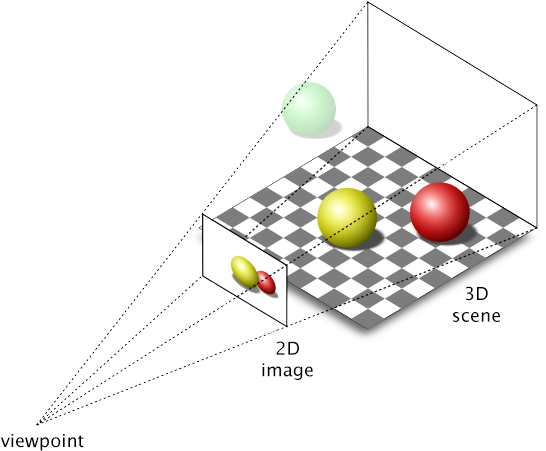
\includegraphics[width=\textwidth]{images/cameraprojection.png}  
  \end{column}
  \begin{column}{0.5\textwidth}
   \begin{itemize}
    \item Light reflects on the surfaces.
    \item The sensor counts the photons.
    \item Objects \textit{occlude} each other.\\
    (Pixels belong to one object.)
    \item Limited field of view.\\
    (Objects appear/disappear.)
   \end{itemize}
  \end{column}
 \end{columns}
\end{frame}

\begin{frame}{Auditory data}
 Microphones capture the air pressure variations.\vspace{3mm}
 \begin{columns}
  \begin{column}{0.5\textwidth}
  \centering
   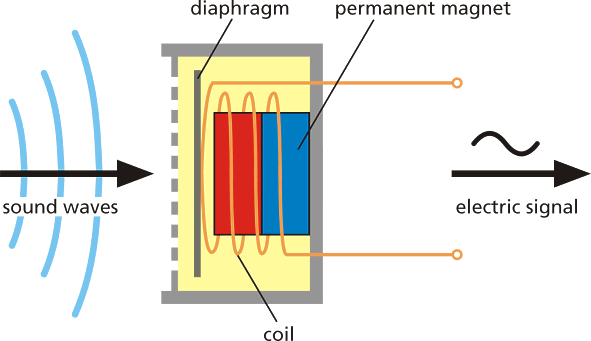
\includegraphics[width=0.8\textwidth]{images/microphone.png}  
  \end{column}
  \begin{column}{0.5\textwidth}
   \begin{itemize}
    \item Sound waves reflect on surfaces.
    \item The sensor measures air pressure variations.
    \item Objects \textit{overlap} each other.\\
    (Sound samples belong to various objects.)
    \item Quasi-omni-directional.
    \item Intermitent activity.
   \end{itemize}
  \end{column}  
 \end{columns}
\end{frame}

\begin{frame}{Audio-visual data}
 How to relate information in different modalities (audio and video)?\\
 \begin{itemize}
  \item Synchronisation
  \item Calibration
  \item Semantic correspondence
 \end{itemize}
  \begin{columns}
  \begin{column}{0.5\textwidth}
  \centering
   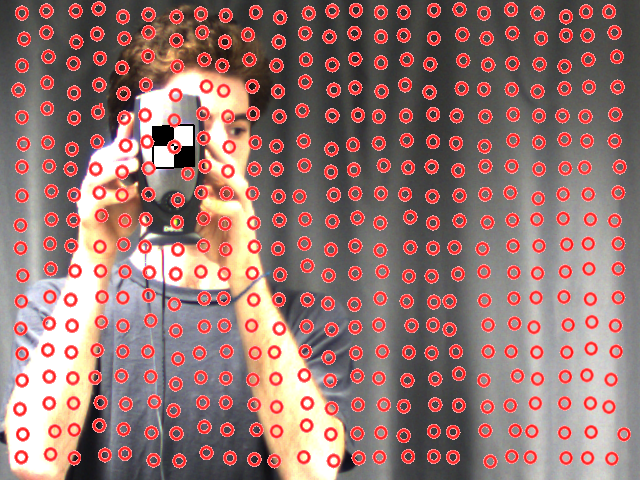
\includegraphics[width=0.65\textwidth]{images/avcalib.png}  
  \end{column}
  \begin{column}{0.5\textwidth}
  \centering
   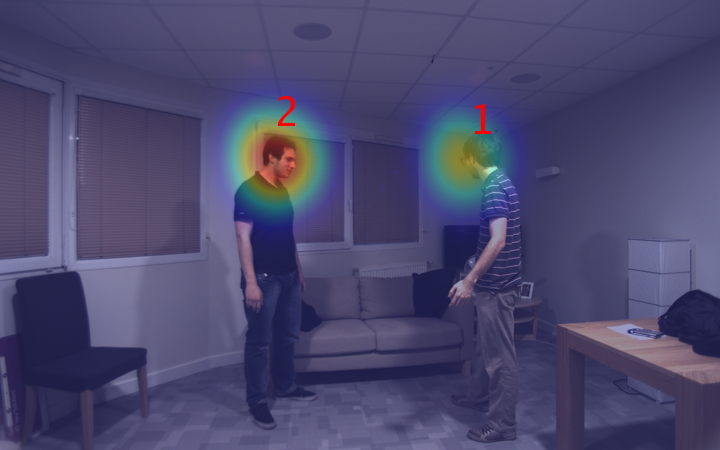
\includegraphics[width=0.8\textwidth]{images/avtracking.png}  
  \end{column}  
 \end{columns}
\end{frame}

\begin{frame}{Challenges in each modality}
 So why using various modalities? Because of their limitations.\vspace{3mm}

%  \begin{columns}
%   \begin{column}{0.8\textwidth}
 Vision:\vspace{-2mm}
 {\small\begin{itemize}
  \item Low resolution if far away.\vspace{-2mm}
  \item Blur, occlusions, variable lighting conditions.\vspace{-2mm}
  \item People/objects cropped/appearing/disappearing.\vspace{-2mm}
  \item Changes in appearance.
 \end{itemize}}

 Audio:\vspace{-2mm}
 {\small\begin{itemize}
  \item Speaker overlap.\vspace{-2mm}
  \item Background noise (and other undesired sources).\vspace{-2mm}
  \item Presence of reverberations.\vspace{-2mm}
  \item Impact of the body on which\\ the microphones are mounted.
 \end{itemize}} 
%   \end{column}
%   \begin{column}{0.2\textwidth}
%   \centering
\vspace{-4cm}
\begin{flushright}
 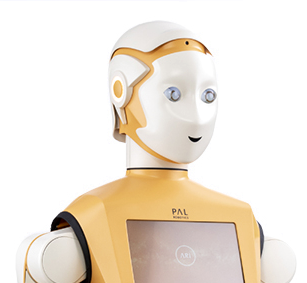
\includegraphics[width=0.35\textwidth]{images/ARIrobot.png}   
\end{flushright}
%   \end{column}  
%  \end{columns}
\end{frame}


\section{Representing Audio Data}

\begin{frame}{The raw data}
  Microphones capture the air pressure variations.\vspace{3mm}
 
  This \textit{continuous} signal is \textit{sampled} into a \textit{discrete} signal.
  \begin{figure}
   \centering
   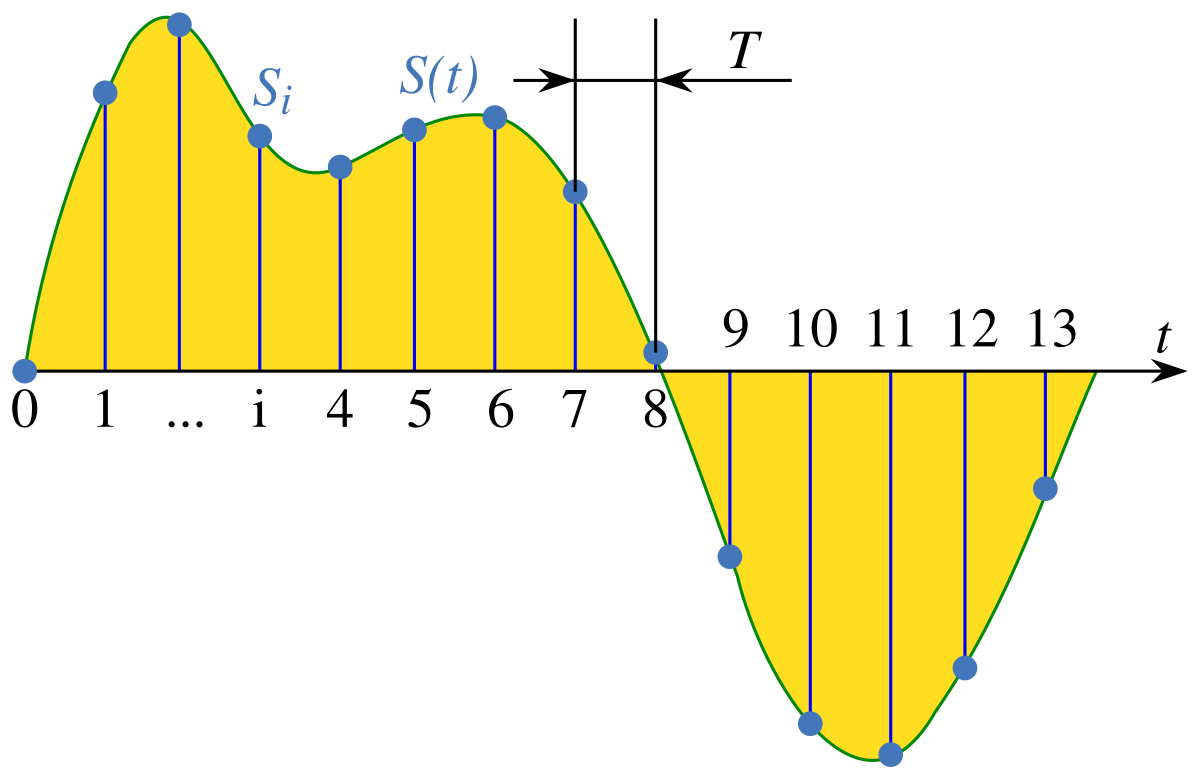
\includegraphics[width=0.7\textwidth]{images/sampling.png}
  \end{figure}

  We never work with $x(t)$ but rather with $x[n]=x(t=nT)$.\\
  Where $T$ is the sampling period.
\end{frame}

\begin{frame}{The Nyquist frequency}
 What is the problem with sampling?
 \begin{figure}
  \centering
  \only<1>{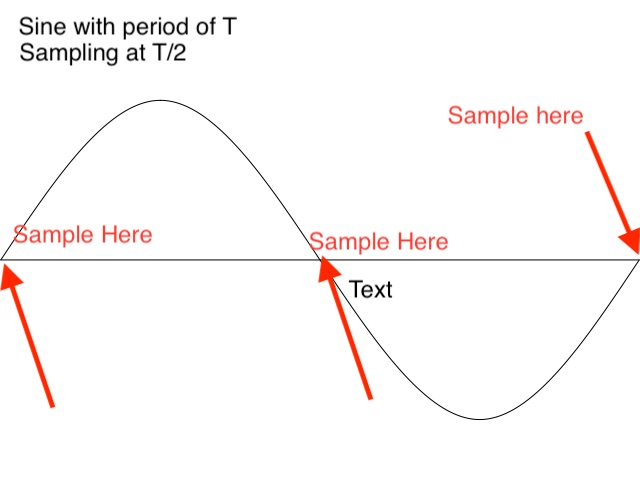
\includegraphics[width=0.5\textwidth]{images/nyquist1.jpg}}%
  \only<2>{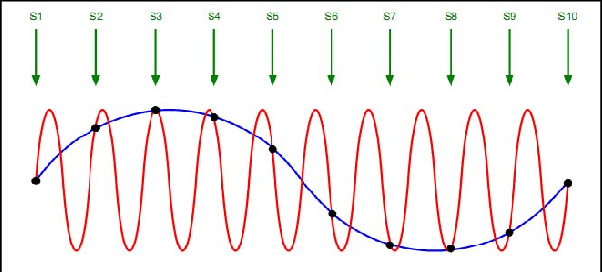
\includegraphics[width=0.5\textwidth]{images/nyquist2.png}}
 \end{figure}
 \only<2>{\begin{block}{Nyquist-Shanon Sampling Theorem}
  If a continuous signal is sampled at a frequency $F_s$, we can only reconstruc the content corresponding to frequencies $<F_s/2$.
 \end{block}}
\end{frame}

\begin{frame}{Every-day example of this}
The phone!
 \begin{itemize}
  \item Speech signal can contain energy up to $20$~kHz.
  \item Most of the energy is within the range $0.3$-$3$~kHz.
  \item This is why the phone standards sample at $8$~kHz.
  \item Keeping most of the content.
  \item Losing high-frequency details - \textit{telephone voice} effect.
 \end{itemize}\vspace{4mm}
Two VERY important operations with discrete signals:
 \begin{itemize}
  \item convolution (as in CNN),
  \item discrete Fourier transform.
 \end{itemize}
\end{frame}
% 
% \begin{frame}{The Convolution}
% 
%   \begin{columns}
%   \begin{column}{0.5\textwidth}
% Convolution requires two signals: the input signal $f$ and the kernel signal $k$.\vspace{3mm}
% 
% The convolution is denoted and defined as:
% \[ (f * g)[n] = \sum_m f[m] g[n-m]. \] 
%   \end{column}
%   \begin{column}{0.5\textwidth}
%   \centering
%    \includegraphics[width=0.6\textwidth]{images/convolution.png}  
%   \end{column}  
%  \end{columns}
% \end{frame}
% 
% \begin{frame}{Convolution Example (you check home)}
%  Example: $f=[7,4,-3,6,-8]$ and $g=[1,1,-1]$.\\
%  {\footnotesize Arrays start at zero: $f[0]=7$, $g[0]=1$.}\vspace{2mm}\\
%  
%  Let's play!\\
%  $(f*g)[0]=\sum_m f[m] g[-m] = 7$\\
%  $(f*g)[1]=\sum_m f[m] g[1-m] = 11$\\
%  $(f*g)[2]=\sum_m f[m] g[2-m] = -6$\\
%  $(f*g)[3]=\sum_m f[m] g[3-m] = -1$\\
%  $(f*g)[4]=\sum_m f[m] g[4-m] = 1$\\
%  $(f*g)[5]=\sum_m f[m] g[5-m] = -14$\\
%  $(f*g)[6]=\sum_m f[m] g[6-m] = 8$\vspace{3mm}\\
%  
%  What is the length of the output signal? $\textrm{len}((f * g)) = \textrm{len}(f) + \textrm{len}(g) - 1$.
% \end{frame}
% 
% \begin{frame}{Properties of the Convolution}
%  Properties:
%  \begin{itemize}
%   \item Linear: $(f*(g+h)) = (f*g) + (f*h)$.
%   \item Associativity: $((f*g)*h) = (f*(g*h))$.
%   \item Commutativity: $(f*g)=(g*f)$.
%   \item ...
%  \end{itemize}\vspace{3mm}
% 
%  
%  Modes:
%  \begin{itemize}
%   \item \textcolor{blue}{Full} (as in the previous slide): all outputs are kept.
%   \item \textcolor{red}{Same} the output has the same length as the input.
%   \item \textcolor{green}{Valid} only outputs involving the full input/kernel signal are kept.
%  \end{itemize}
%  \[(f*g) = [\underbrace{7,\underbrace{11,\underbrace{-6,-1,1}_{\textcolor{green}{Valid}},-14}_{\textcolor{red}{Same}},8}_{\textcolor{blue}{Full}}]\]
% \end{frame}
% 
% \begin{frame}{The 2D \& 3D Convolution}
%  Higher dimensional versions of the convolution operator exist: \vspace{3mm}
%    \begin{columns}
%   \begin{column}{0.5\textwidth}
%    \centering
%    \includegraphics[width=0.8\textwidth]{images/2dconvolution.png}  
%   \end{column}
%   \begin{column}{0.5\textwidth}
%   \centering
%    \includegraphics[width=0.8\textwidth]{images/3dconvolution.png}  
%   \end{column}  
%  \end{columns}\vspace{3mm}
%  
%  In which ``mode'' are these schemes? (Full, Same, Valid)
% \end{frame}

\begin{frame}{The discrete Fourier transform}
 Purpose: structure the information in frequencies instead of time.\vspace{2mm}\\
 Input: signal in the time domain $f[0],\ldots,f[L-1]$.\vspace{2mm}\\
 Output: a sequence of $L$ complex numbers describing the magnitude and phase at each frequency bin.\vspace{2mm}\\
 Formula: \[F[k] = \sum_{n=0}^{L-1} f[n] \exp\left(-i\frac{2\pi}{L}kn\right).\]
 Fast Fourier transform (FFT): an efficient algorithm to compute DFT when $L$ is a power of 2.
\end{frame}

\begin{frame}{The discrete Fourier transform (II)}
 Fourier domain decomposes the signal in frequencies not in time:\\
 \begin{figure}
  \centering
  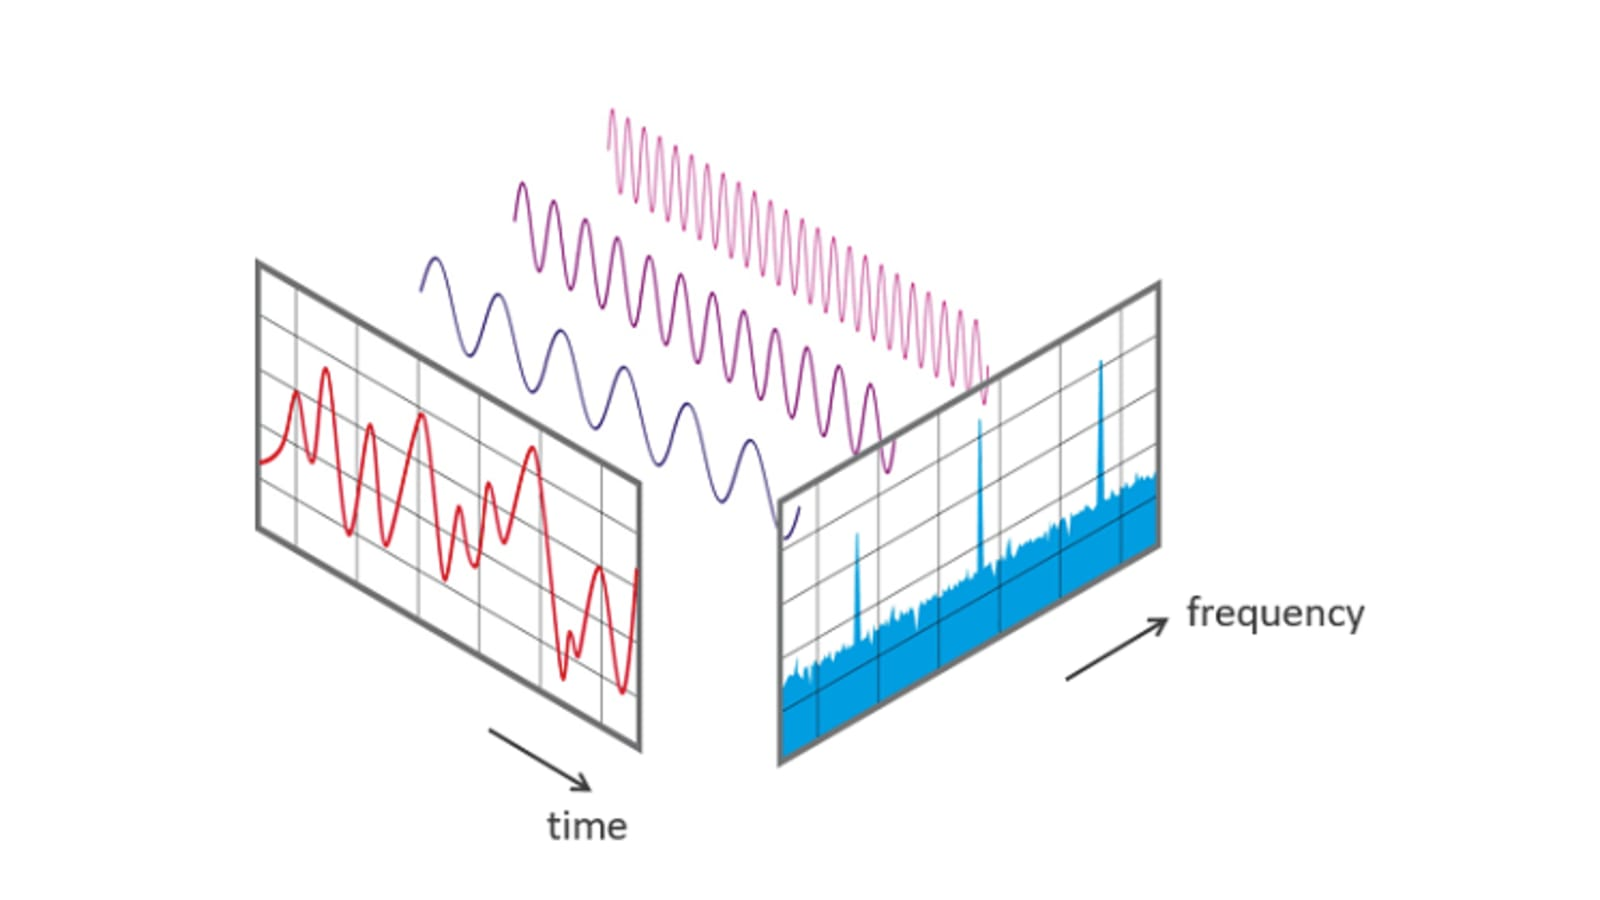
\includegraphics[width=0.8\textwidth]{images/fourierdomain.png}
 \end{figure}
 Problem: we have to choose either time \textit{or} frequency.
\end{frame}

\begin{frame}{The short-time Fourier transform}
 STFT: segment the input signal, and apply DFT to each segment.
\begin{figure}
\centering
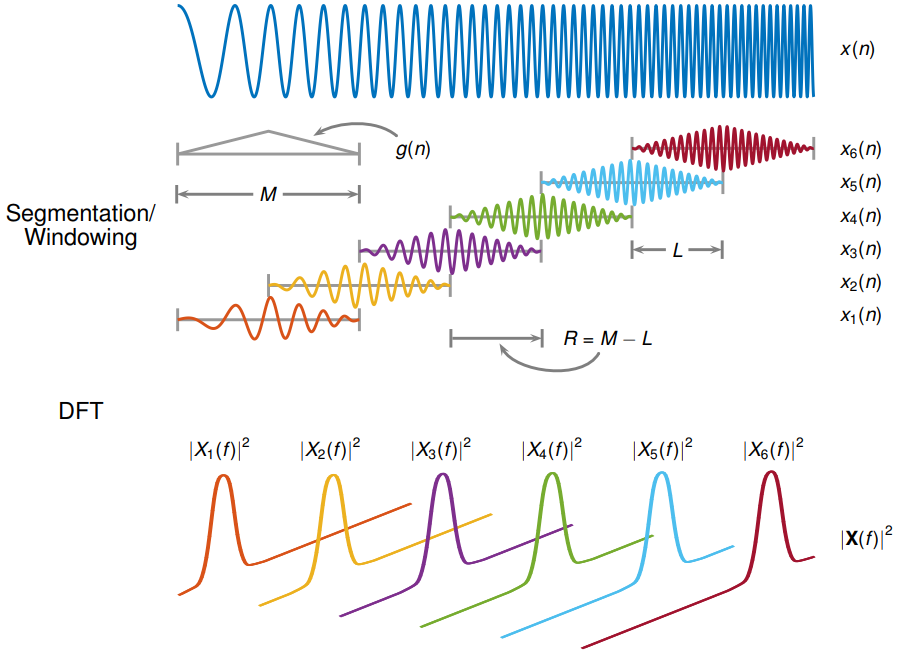
\includegraphics[width=0.65\textwidth]{images/stft.png}
\end{figure}

\alert{Let's check that with a nice wav file!}
\end{frame}

\begin{frame}{STFT comments}
 \begin{itemize}
  \item There is a duality:
  \begin{itemize}
   \item Represent the frequential content at a given time.
   \item Represent the evolution of a given frequency over time.
  \end{itemize}\vspace{3mm}
  \item STFT requires to \textit{window} the signal with a kernel.\\
  Different kernels lead to different properties (e.g.\ reconstruction).\vspace{3mm}
  \item Other parameters: the window length and overlap.\\
  They provide the rate of frequency vectors (DFT outputs).\\
  If correctly chosen the correspond to, e.g.\ video frames.\vspace{3mm}
 \end{itemize}
    \centering
    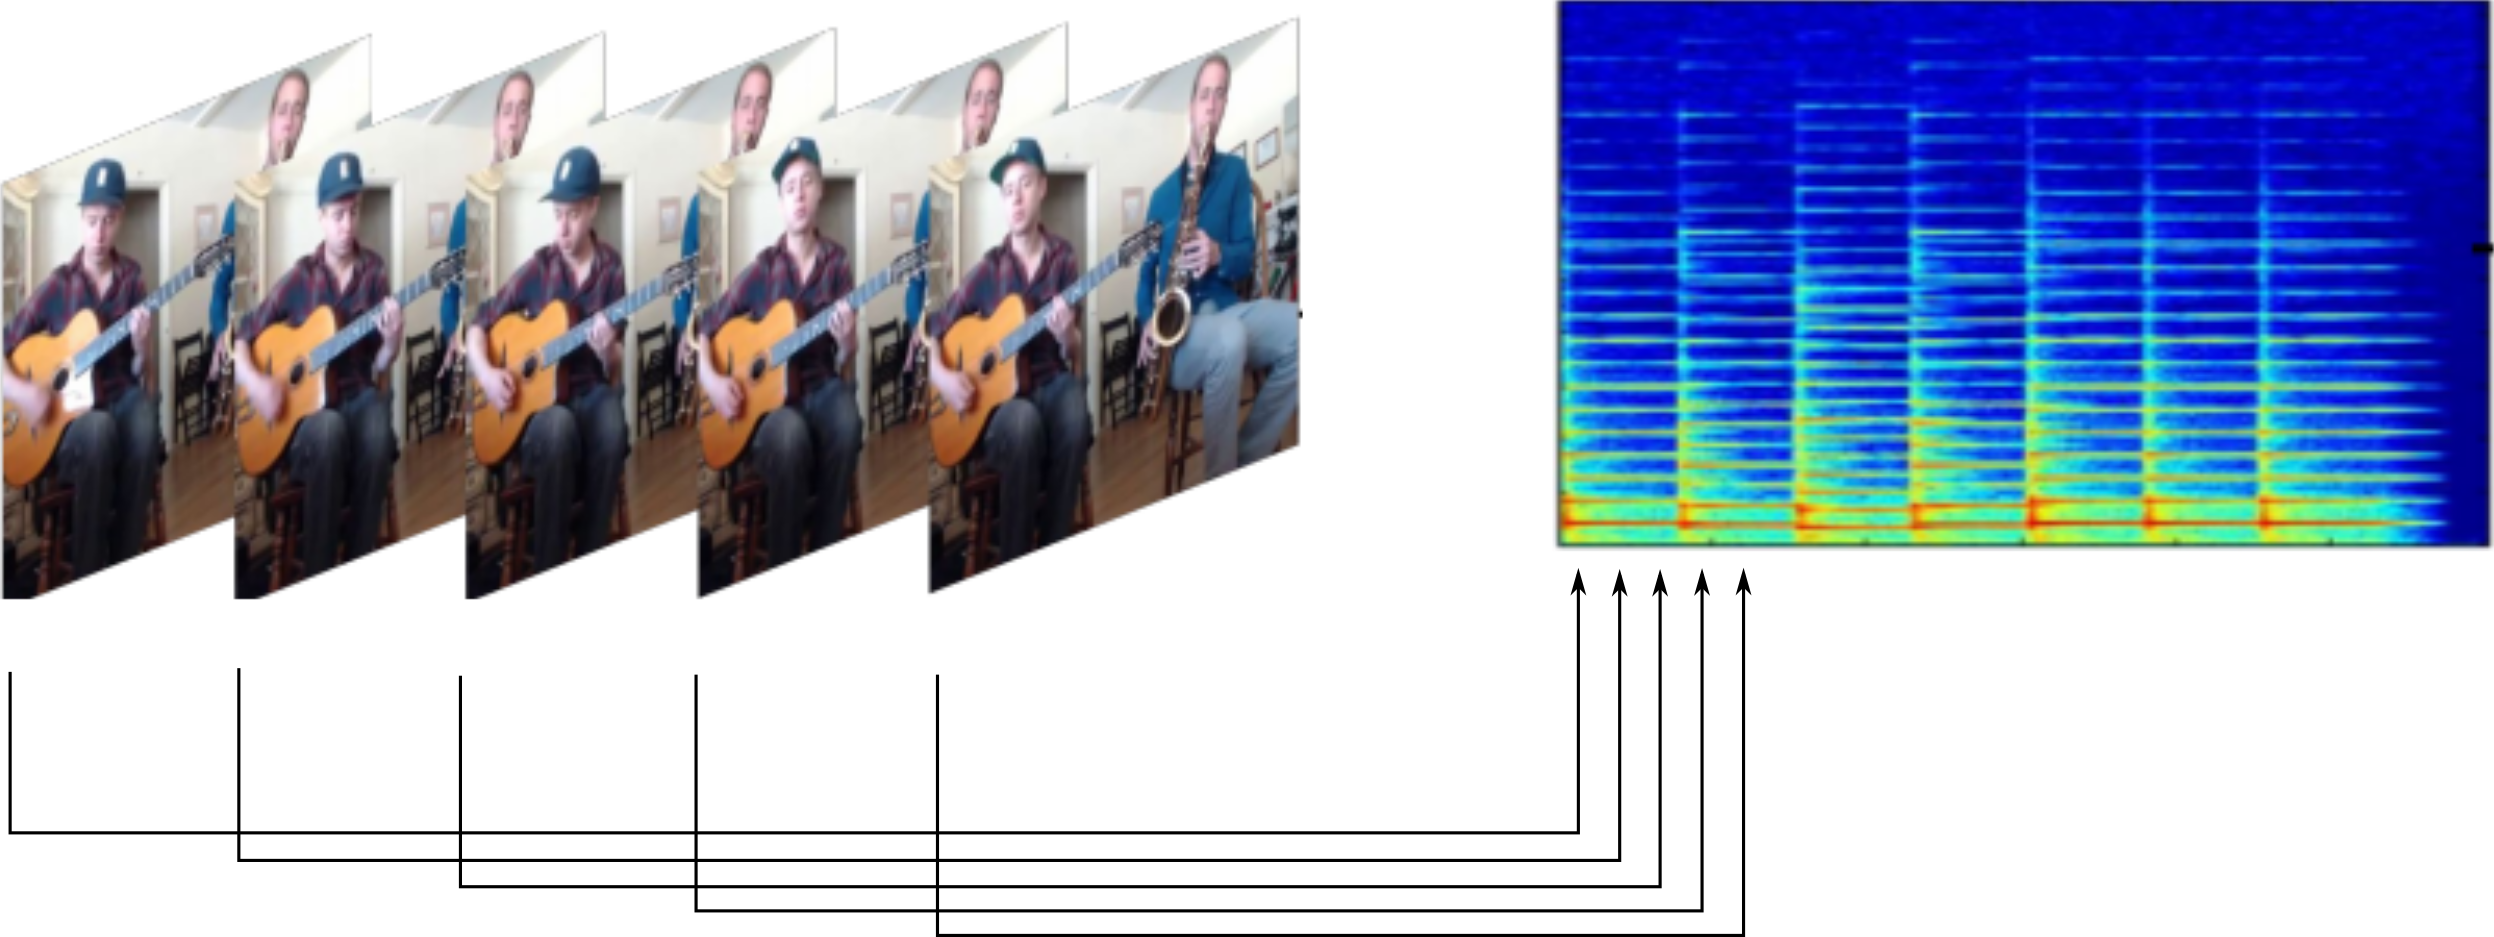
\includegraphics[width=0.5\textwidth]{images/avcorrespondence.png}
\end{frame}


\begin{frame}{Let's \textit{see} it!}
\begin{itemize}
 \item Sine frequency sweep (pure sine of increasing frequency).
 \item Leyenda (piano, harmonics).
 \item O mio babbino caro (opera, vibrato).
 \item Highway to hell (rock\& roll, distortion).
\end{itemize}
\end{frame}


%%%%%%%%%%%%%%%%%%%%%%%%%%%%%%%%%%%%%%%%%%%%%%%%%%%%%%%%%%%%%%
\section{Learning with Audio-Visual Data}
%%%%%%%%%%%%%%%%%%%%%%%%%%%%%%%%%%%%%%%%%%%%%%%%%%%%%%%%%%%%%%

\begin{frame}{Background}
\begin{itemize}
 \item AV Processing is moderately old (started on 2000's).
 \item Deep learning and data availability offer a new perspective to these tasks.
 \item Yet, data is not available for all AV tasks, and we often need to simulate.\\
 Realistic AV simulation of social scenes is also difficult.
\end{itemize}

\centerimage{0.5}{images/AVLocalisation-3.png}
\end{frame}

\begin{frame}{Learn to separate sounds {\small [Gao et al, ECCV 2018]}}
 \centerimage{1}{images/LearnToSeparateTeaser.png}
 
 Given two input videos and a mixed monaural (1 mic) audio, can we separate the  signals?
\end{frame}

\begin{frame}{Learn to separate sounds (II) {\small [Gao et al, ECCV 2018]}}
 \centerimage{1}{images/LearnToSeparateArch.png}
  \begin{itemize}
   \item Visual features from pre-trained ResNet.
   \item Audio features from non-negative matrix factorisation.
   \item Associate those through multi-instance multi-label learning.
  \end{itemize}

\end{frame}

\begin{frame}{Non-negative matrix factorisation?}
 \centerimage{0.7}{images/nmf_en.png}
 {\small [Image from \url{http://d-kitamura.net/demo-defNMF_en.html}]}
\end{frame}


\begin{frame}{Learn to separate sounds (III) {\small [Gao et al, ECCV 2018]}}
 Main idea:
 \begin{itemize}
  \item Learn a set of sound ``basis'' to represent the spectrogram of each instrument.
  \item Use vision to select the right instrument from the visual appearance.
 \end{itemize}
 
 \centerimage{1}{images/VisionToNMFSelection.png}
\end{frame}
%
% \begin{frame}{What if we have two microphones? {\small [Gao et al, ICCV 2019]}}
%   \centerimage{0.6}{images/25DSoundTeaser.png}
%   Can we \textit{spatialise} the sound with visual guidance?
% \end{frame}
%
% \begin{frame}{What if we have two microphones? (II) {\small [Gao et al, ICCV 2019]}}
%   \begin{columns}
%    \begin{column}{0.5\textwidth}
%        \centerimage{1}{images/25DSoundRecordingSetup.png}
%    \end{column}
%    \begin{column}{0.5\textwidth}
%         We need data!!!
%
%         \begin{itemize}
%          \item Specific AV recording device.
%          \item Emulating human ear.
%          \item Various instruments playing.
%         \end{itemize}
%
%    \end{column}
%   \end{columns}
% \end{frame}
%
% \begin{frame}{What if we have two microphones? (III) {\small [Gao et al, ICCV 2019]}}
%   \centerimage{0.8}{images/25DSoundArchitecture.png}
%   Extract visual features (ResNet) and concatenate with the bottleneck of a U-Net.\\
%   Learn \textbf{only} the U-Net.
% \end{frame}
%
% \begin{frame}{What if we have two microphones? (IV) {\small [Gao et al, ICCV 2019]}}
% %   \begin{columns}
% %    \begin{column}{0.5\textwidth}
%        \centerimage{0.7}{images/25DSound-MixSeparate.png}
% %    \end{column}
% %    \begin{column}{0.5\textwidth}
%         Downstream task: binaural sound separation. Evaluate with the mix-and-separate strategy.
% %    \end{column}
% %   \end{columns}
% \end{frame}

\begin{frame}{Can we separate voice? (back to single microphone) {\small [Gao et al, CVPR 2021]}}
 Instruments have very different visual and audio signatures, but voices/faces have less variance.
 \centerimage{0.6}{images/VisualVoiceTeaser.png}
\end{frame}

\begin{frame}{Can we do that with voice? (II) {\small [Gao et al, CVPR 2021]}}
 \centerimage{0.6}{images/VisualVoiceArchitecture.png}
 Similar U-Net architecture, but:
 \begin{itemize}
  \item We need to fuse face and lip features.
  \item Lip information changes over time.
 \end{itemize}
\end{frame}

\begin{frame}{Can we do that with voice? (III) {\small [Gao et al, CVPR 2021]}}
 \centerimage{0.9}{images/VisualVoiceFulllArch.png}
%  Similar U-Net architecture, but:
%  \begin{itemize}
%   \item We need to fuse face and lip features.
%   \item Lip information changes over time.
%  \end{itemize}
\end{frame}
%
% \begin{frame}{Example of downstream tasks}
%    \begin{itemize}
%   \item AV sound source localisation.
%   \item AV Robot navigation \& planning.
%  \end{itemize}\vspace{3mm}
%
%   \begin{columns}
%    \begin{column}{0.3\textwidth}
%       \centerimage{1}{images/AVLocalisation-1.png}
%    \end{column}
%    \begin{column}{0.3\textwidth}
%       \centerimage{1}{images/AVLocalisation-2.png}
%    \end{column}
%    \begin{column}{0.3\textwidth}
%       \centerimage{1}{images/AVLocalisation-4.png}
%    \end{column}
%  \end{columns}\vspace{3mm}
%
%
%  {\small [Chen et al, ECCV 2020, CVPR 2021]}
% \end{frame}

%%%%%%%%%%%%%%%%%%%%%%%%%%%%%%%%%%%%%%%%%%%%%%%%%%%%%%%%%%%%%%
\section{Unsupervised Adaptation with Audio-Visual Data}
%%%%%%%%%%%%%%%%%%%%%%%%%%%%%%%%%%%%%%%%%%%%%%%%%%%%%%%%%%%%%%

%%%%%%%%%%%%%%%%%%%%%%%%%%%%%%%%%%%%%%%%%%%%%%%%%%%%%%%%%%%%%%%%%%%%%%%%%%%%
\begin{frame}{What is Speech Enhancement}


\centering
Speech Enhancement: Remove the background noise from the observed mixture speech.

\begin{figure}
\centering
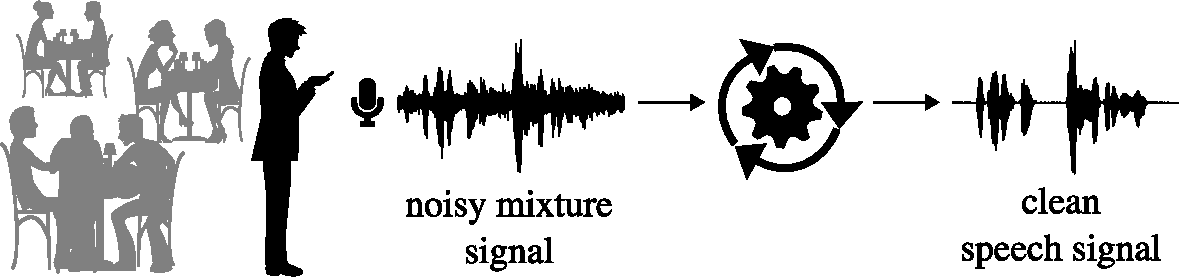
\includegraphics[scale=0.4]{images/intro_speech_enhancement.pdf}
\end{figure}

%\pause
Short-time Fourier transform (STFT): time-frequency matrix representation.
\begin{figure}
\centering
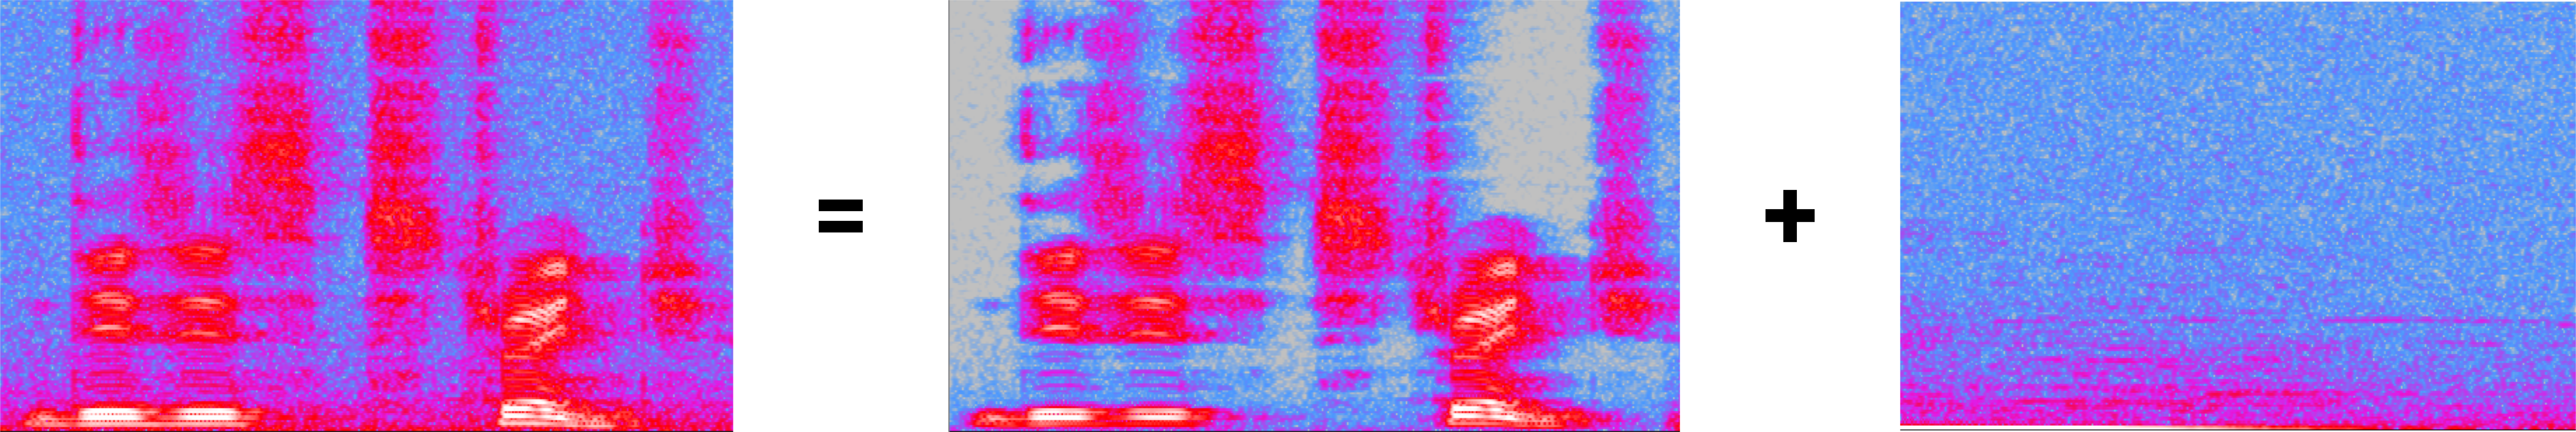
\includegraphics[width=0.8\textwidth]{images/spectrogram.png}
\end{figure}
\vspace{-6mm}
\begin{equation*}
\underbrace{\mathbf{x}}_{\text{Noisy mixture}} \quad\qquad=\quad\qquad \underbrace{\mathbf{s}}_{\text{Clean speech}} \quad\qquad+\quad\qquad \underbrace{\mathbf{b}}_{\text{Noise signal}}
\end{equation*}
% \textbf{Task}: Given $\mathbf{x}$ we want an estimate $\hat{\mathbf{s}}$.
\end{frame}

%%%%%%%%%%%%%%%%%%%%%%%%%%%%%%%%%%%%%%%%%%%%%%%%%%%%%%%%%%%%%%%%%%%%%%%%%%%%
\begin{frame}{Audio-visual Speech Enhancement (AV-SE)}

\begin{itemize}
	\item {Visual data, i.e. \alert{lips movements}, provides some complementary information about the unknown speech.}
	\item For \alert{highly noisy audio recordings}, visual information can be very helpful.
\end{itemize}

\begin{center}
	\begin{figure}
		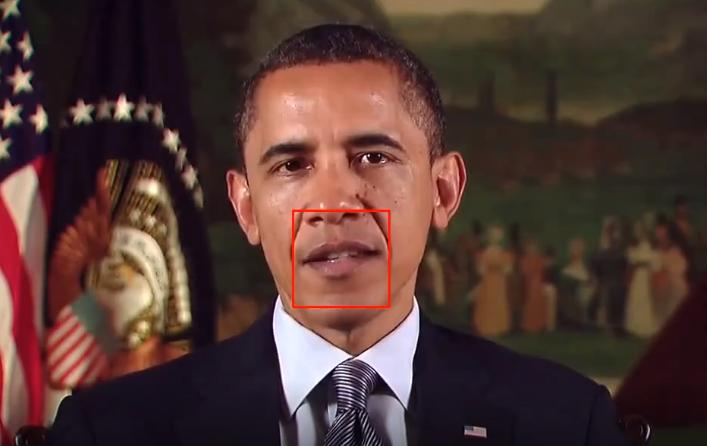
\includegraphics[scale=0.2]{images/obama.png}
	\end{figure}
\end{center}
%\pause
How to efficiently fuse audio and visual modalities for speech enhancement?
\end{frame}

%%%%%%%%%%%%%%%%%%%%%%%%%%%%%%%%%%%%%%%%%%%%%%%%%%%%%%%%%%%%%%%%%%%%%%%%%%%%
\begin{frame}{Supervised vs.\ Unsupervised AVSE}
	\textbf{Supervised:} Learn a mapping to denoise audio data [Gabbby et al., 2018]:
	\begin{center}
		\begin{figure}
			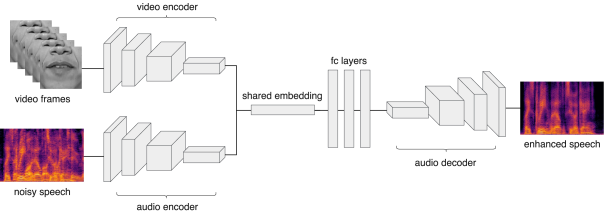
\includegraphics[scale=0.4]{images/supervised_se.png}
		\end{figure}
	\end{center}
%\pause
	\textbf{Unsupervised Adaptation:} Learn a \alert{generative audio-visual model for clean speech} and combine it with an \alert{unsupervised noise model} at test time.\vspace{5mm}

	Unsupervised SE is \textbf{more appropriate in robotics} since the noise type is unknown.
\end{frame}

%%%%%%%%%%%%%%%%%%%%%%%%%%%%%%%%%%%%%%%%%%%%%%%%%%%%%%%%%%%%%%%%%%%%%%%%%%%%
\begin{frame}{Unsupervised speech enhancement: overview}
\textbf{Train} a \alert{generative speech model} with clean data: $\{\mathbf{s}_i\}_{i=1}^N$.

\begin{center}
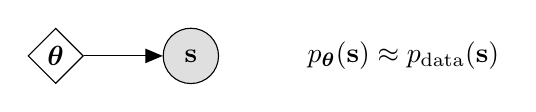
\begin{tikzpicture}
        \node[det] (theta) {\alert{$\bs{\theta}$}};
        \node[obs,right=of theta] (s) {$\mathbf{s}$};
        \node[right=of s] (disc) {$p_{\bs{\theta}}(\mathbf{s})\approx p_{\text{data}}(\mathbf{s})$};
        \edge{theta} {s};
\end{tikzpicture}
\end{center}
\pause


\textbf{Adaptation/test}: learn the \alert{noise parameters} of $\mathbf{x}$:

\begin{center}
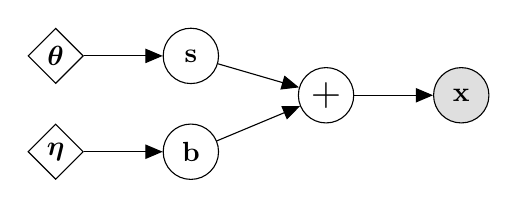
\begin{tikzpicture}
        \node[det] (theta) {$\bs{\theta}$};
        \node[latent,right=of theta] (s) {$\mathbf{s}$};
        \node[det,below=of theta,yshift=5mm] (eta) {$\alert{\bs{\eta}}$};
        \node[latent,right=of eta] (b) {$\mathbf{b}$};
        \node[latent,right=of s,yshift=-5mm] (plus) {\Large$+$};
        \node[obs,right=of plus] (x) {$\mathbf{x}$};
        \edge{theta} {s};
        \edge{eta} {b};
        \edge{s,b} {plus};
        \edge{plus} {x};
\end{tikzpicture}
\end{center}

We start with the ``train'' phase (we'll see the adaptation if we have time).
\end{frame}


%%%%%%%%%%%%%%%%%%%%%%%%%%%%%%%%%%%%%%%%%%%%%%%%%%%%%%%%%%%%%%%%%%%%%%%%%%%%
\begin{frame}{Interest of probabilistic learning?}
 Probabilistic generative models aim to learn a (parametric) \emph{distribution} $p_{\bs{\theta}}(\bs{x})$ that approximates the complex data distribution $ p_{\text{\tiny{data}}}(\bs{x})$:
\begin{figure}
\centering
    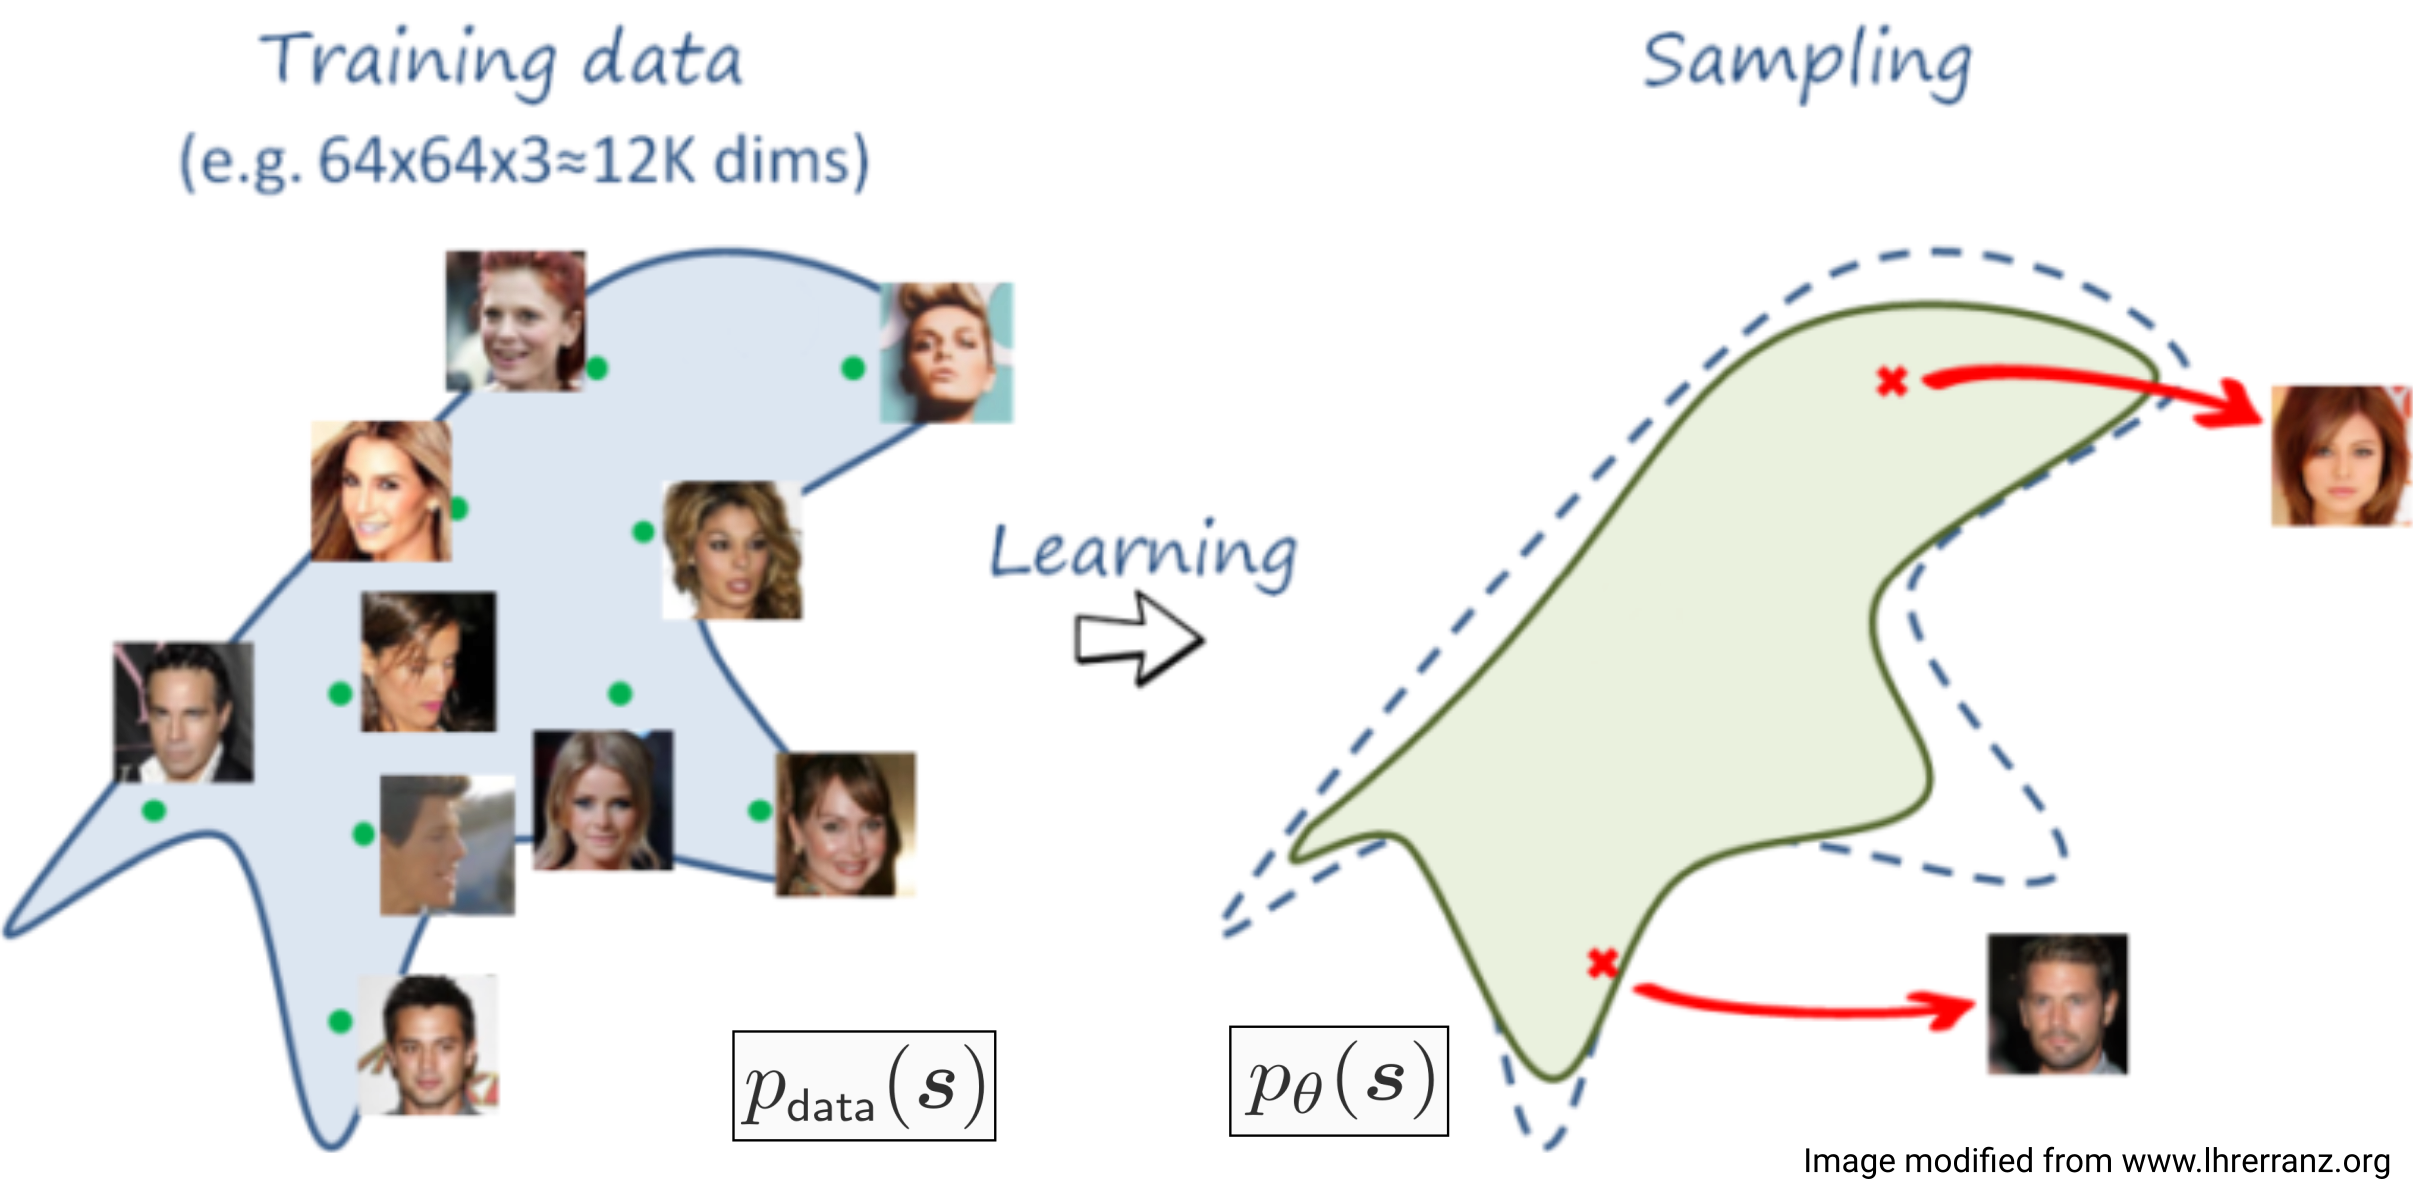
\includegraphics[scale=0.45]{images/generative-model-mod.png}
\end{figure}

% Probabilistic models are interesting because:
\begin{itemize}
 \item Once learned, we can (ideally) sample new data.
 \item We can jointly learn them with other probabilistic models using \textit{maximum likelihood}.
\end{itemize}
\end{frame}

%%%%%%%%%%%%%%%%%%%%%%%%%%%%%%%%%%%%%%%%%%%%%%%%%%%%%%%%%%%%%%%%%%%%%%%%%%%%
\begin{frame}{The Kullback-Leibler divergence and the ML formulation}
The Kullback-Leilbler (KL) divergence between two distributions writes:
\begin{equation*}
 D_{\text{KL}}(p(\bs{x})\|q(\bs{x})) = -\E_{p(\bs{x})}\left[\log\frac{q(\bs{x})}{p(\bs{x})}\right] = -\int_{\cal X} p(\bs{x})\log\frac{q(\bs{x})}{p(\bs{x})}\textrm{d}\bs{x} \left\{\begin{array}{l} \geq 0 \\ \neq D_{\text{KL}}(q(\bs{x})\|p(\bs{x})) \end{array}\right.
\end{equation*}
$D_{\text{KL}}(p(\bs{x})\|q(\bs{x})) = 0 \Leftrightarrow p(\bs{x})=q(\bs{x})$.\vspace{10mm}\\

\pause
Given a training set $\{\bs{x}_i\}_{i=1}^N, \bs{x}_i\sim p_{\text{\tiny{data}}}(\bs{x})$, ML minimizes the KL divergence:
\begin{align*}
\bs{\theta}^*=&\argmin_{\bs{\theta}}~ D_{\text{KL}}\Big(p_{\text{\tiny{data}}}(\bs{x}) \parallel p_{\bs{\theta}}(\bs{x})\Big)=\argmin_{\bs{\theta}}~-\E_{p_{\text{\tiny{data}}}}\Big[ \log \frac{p_{\bs{\theta}}(\bs{x})}{p_{\text{\tiny{data}}}(\bs{x})}\Big]\\
=& \argmax_{\bs{\theta}}~\E_{p_{\text{\tiny{data}}}}\Big[ \log {p_{\bs{\theta}}(\bs{x})}\Big]
\approx \boxed{\argmax_{\bs{\theta}}~{\frac{1}{N}\sum_{i=1}^N \log {p_{\bs{\theta}}(\bs{x}_i)}}}
\end{align*}
\end{frame}

%%%%%%%%%%%%%%%%%%%%%%%%%%%%%%%%%%%%%%%%%%%%%%%%%%%%%%%%%%%%%%%%%%%%%%%%%%%%
\begin{frame}{Interest of Latent Variables}
\begin{itemize}
 \item Speech enhancement: noisy speech (observation), clean speech (latent variable)
%  $\rightarrow$ Get rid of noise heard together with speech.
 \item Person tracking: detections (observation), person positions (latent variable)
%  $\rightarrow$ Track occluded persons, filter over time.
 \item Representation learning: raw data (observation), representation (latent variable)
%  $\rightarrow$ Compute an optimal compact representation of the raw data.
\end{itemize}\pause

Let $\bs{z}$ denote the latent variable:
\[
\begin{cases}
\bs{z}\sim p_{\bs{\theta}}(\bs{z})\\
\bs{x}|\bs{z}\sim p_{\bs{\theta}}(\bs{x}|\bs{z})
\end{cases}\rightarrow~ p_{\bs{\theta}}(\bs{x})=\int p_{\bs{\theta}}(\bs{x}, \bs{z}) \textrm{d}\bs{z} = \int p_{\bs{\theta}}(\bs{x}|\bs{z})p_{\bs{\theta}}(\bs{z}) \textrm{d}\bs{z}\]

\pause
\textbf{New samples:} Draw $ \hat{\bs{z}} \sim p_{\bs{\theta}}(\bs{z}) $, then draw a new sample $ \hat{\bs{x}} \sim p_{\bs{\theta}}(\bs{x}|\hat{\bs{z}}) $.

\textbf{Learning:} How to estimate $\bs{\theta}$ with the ML formulation?

\textbf{Inference:} How to get the most likely latent $p_{\bs{\theta}}(\bs{z}
|\bs{x})$?
\end{frame}

%%%%%%%%%%%%%%%%%%%%%%%%%%%%%%%%%%%%%%%%%%%%%%%%%%%%%%%%%%%%%%%%%%%%%%%%%%%%
\begin{frame}{The Gaussian Mixture Model (GMM)}
Definition:
\begin{itemize}
 \item For each $\bs{x}_n$ there is a latent variable $\bs{z}_n$ taking values from 1 to $K$: $\bs{z}_n\in\{1,\ldots,K\}$.\pause
 \item Its prior probability is defined as: $p(\bs{z}_n=k)=\pi_k\geq0$, with $\sum_{k=1}^K \pi_k = 1$.\pause
 \item Given $z_n$, the data point is modeled as a multivariate Gaussian:\vspace{-2mm}
 \[p(\bs{x}_n|\bs{z}_n=k) = \mathcal{N}(\bs{x}_n;\bs{\mu}_k,\bs{\Sigma}_k) \]
\end{itemize}
% \vspace{3mm}
Advantages:
 \begin{enumerate}
  \item Having $\pi_1,\ldots,\pi_K$ means that groups can be differently populated.
  \item The shape of the groups is modeled by $\bs{\Sigma}_k$.
  \item The parameters are: {\color{orange}$\bs{\theta}=\{\pi_k,\bs{\mu}_k,\bs{\Sigma}_k\}_{k=1}^K$}.
 \end{enumerate}
\end{frame}

%%%%%%%%%%%%%%%%%%%%%%%%%%%%%%%%%%%%%%%%%%%%%%%%%%%%%%%%%%%%%%%%%%%%%%%%%%%%
\begin{frame}{Maximum likelihood for GMM}
 Let's compute $p(\bs{x}_n)$
 \[ p(\bs{x}_n) = \sum_{k=1}^K p(\bs{x}_n,\bs{z}_n=k) = \sum_{k=1}^K \pi_k\mathcal{N}(\bs{x}_n;\bs{\mu}_k,\bs{\Sigma}_k).\]
 The log-likelihood:
 \[\mathcal{L}(\bs{\theta}|\bs{X}) = \sum_{n=1}^N \log  \sum_{k=1}^K \pi_k\mathcal{N}(\bs{x}_n;\bs{\mu}_k,\bs{\Sigma}_k),\]

 Computing directly ML by $\displaystyle\frac{\partial\mathcal{L}}{\partial\pi_k}=0$, $\displaystyle\frac{\partial\mathcal{L}}{\partial\bs{\mu}_k}=0$ or $\displaystyle\frac{\partial\mathcal{L}}{\partial\bs{\Sigma}_k}=0$ is very difficult.
\end{frame}

%%%%%%%%%%%%%%%%%%%%%%%%%%%%%%%%%%%%%%%%%%%%%%%%%%%%%%%%%%%%%%%%%%%%%%%%%%%%
%%%%%%%%%%%%%%%%%%%%%%%%%%%%%%%%%%%%%%%%%%%%%%%%%%%%%%%%%%%%%%%%%%%%%%%%%%%%
% \section{EM for GMM and beyond}

%%%%%%%%%%%%%%%%%%%%%%%%%%%%%%%%%%%%%%%%%%%%%%%%%%%%%%%%%%%%%%%%%%%%%%%%%%%%
\begin{frame}{(Expected complete-data) log-likelihood}
 We have seen that $\log p(\bs{x})$ does not work well with derivatives. However, $\log p(\bs{x},\bs{z})$ does!\vspace{3mm}\\

 \textbf{Problem}: $\bs{z}$ is not observed, thus $\sum_n\log p(\bs{x}_n,\bs{z}_n)$ is a random variable.\vspace{6mm}\\
 \pause

 Given an initial value of the parameters, $\bs{\theta}^0$, let's take the expectation w.r.t.\ the posterior distribution $p(\bs{z}|\bs{x},\bs{\theta}^0)$ {\footnotesize [we will justify this choice later on]}:
 \[\mathcal{Q}(\bs{\theta},\bs{\theta}^0) = \sum_n \mathbb{E}_{p(\bs{z}_n|\bs{x}_n;\bs{\theta}^0)} \log p(\bs{x}_n,\bs{z}_n;\bs{\theta})\]

 This function is called: \textit{expected complete-data log-likelihood}, and is the main mathematical object when working with EM algorithms.
\end{frame}

%%%%%%%%%%%%%%%%%%%%%%%%%%%%%%%%%%%%%%%%%%%%%%%%%%%%%%%%%%%%%%%%%%%%%%%%%%%%
\begin{frame}{The EM algorithm for GMM}
 Given $\bs{\theta}^0$, we use the \textit{expected complete-data log-likelihood} $\mathcal{Q}$. For iteration $r=1,\ldots,R$:\vspace{2mm}
 \begin{enumerate}
  \item Expectation [E-step]:
  \[ \mathcal{Q}(\bs{\theta},\bs{\theta}^{r-1}) = \mathbb{E}_{p(\bs{z}|\bs{x};\bs{\theta}^{r-1})} \log p(\bs{x},\bs{z};\bs{\theta})\]\vspace{-5mm}
  \item Maximisation [M-step]:
  \[ \bs{\theta}^r = \arg\max_{\bs{\theta}} \mathcal{Q}(\bs{\theta},\bs{\theta}^{r-1})\]
 \end{enumerate}
 {\footnotesize (observations $\bs{x}=\{\bs{x}_n\}_{n=1}^N$, latent variables $\bs{z}=\{\bs{z}_n\}_{n=1}^N$, parameters $\bs{\theta}=\{\pi_k,\bs{\mu}_k,\bs{\Sigma}_k\}_{k=1}^K$)}%\pause\vspace{4mm}

%   We can look back to $K$-means:
%  \begin{enumerate}
%   \item Infer latent variables (assignment) given the parameters (centroids) [E-step].
%   \item Estimate the parameters (centroids) given the assignments [M-step].
%  \end{enumerate}
\end{frame}

%%%%%%%%%%%%%%%%%%%%%%%%%%%%%%%%%%%%%%%%%%%%%%%%%%%%%%%%%%%%%%%%%%%%%%%%%%%%
\begin{frame}{The EM algorithm for GMM (II)}
\textbf{E-step} The posterior distribution writes:
\begin{equation*}
 p(\bs{z}_n=k|\bs{x}_n;\bs{\theta}^0) = \frac{p(\bs{z}_n=k;\bs{\theta}^0)p(\bs{x}_n|\bs{z}_n=k;\bs{\theta}^0)}{\sum_\ell p(\bs{z}_n=\ell;\bs{\theta}^0)p(\bs{x}_n|\bs{z}_n=\ell;\bs{\theta}^0)} =  \frac{\pi_k^0\mathcal{N}(\bs{x}_n;\bs{\mu}_k^0,\bs{\Sigma}_k^0)}{\sum_{\ell}\pi_\ell^0\mathcal{N}(\bs{x}_n;\bs{\mu}_\ell^0,\bs{\Sigma}_\ell^0)} = \eta_{nk}
\end{equation*}\pause

The expected complete-data log-likelihood writes:
\begin{equation*}
 \mathcal{Q}(\bs{\theta},\bs{\theta}^0) = \sum_{n=1}^N\sum_{k=1}^K \eta_{nk} \log \pi_k\mathcal{N}(\bs{x}_n;\bs{\mu}_k,\bs{\Sigma}_k)
\end{equation*}\pause

\textbf{M-step} The optimal value for $\bs{\mu}_k$ writes:
  \[\bs{\mu}_k^*=\frac{1}{\sum_{n=1}^N \eta_{nk}}\sum_{n=1}^N\eta_{nk}\bs{x}_n\]
\end{frame}

%%%%%%%%%%%%%%%%%%%%%%%%%%%%%%%%%%%%%%%%%%%%%%%%%%%%%%%%%%%%%%%%%%%%%%%%%%%%
\begin{frame}{But why does the EM work?}
 The main mathematical object in EM is $\mathcal{Q}$ {\footnotesize (The expected complete-data log-likelihood)}.\vspace{4mm}\\

 What is the relationship with the log-likelihood? Let's take any distribution of $\bs{z}$, $q(\bs{z})$:
%  \begin{align*}
% \log p(\bs{x})&= \mathbb{E}_{q(\bs{z})}\Big[\log p(\bs{x})\Big]\\
% &= \mathbb{E}_{q(\bs{z})}\Big[\log p(\bs{x})\frac{p(\bs{z}|\bs{x})q(\bs{z})}{p(\bs{z}|\bs{x})q(\bs{z})}\Big]\\
% &= \underbrace{\mathbb{E}_{q(\bs{z})}\Big[\log \frac{p(\bs{x})p(\bs{z}|\bs{x})}{q(\bs{z})}\Big]}_{\text{M-step - }\mathcal{Q}} +  \underbrace{D_{\text{KL}}\Big(q(\bs{z})\Big\lVert p(\bs{z}|\bs{x})\Big)}_{\text{E-step - KL}}
% \end{align*}
\begin{equation*}
 \log p(\bs{x}) = \underbrace{\mathbb{E}_{q(\bs{z})}\Big[\log \frac{p(\bs{x})p(\bs{z}|\bs{x})}{q(\bs{z})}\Big]}_{\text{M-step - }\mathcal{Q}} +  \underbrace{D_{\text{KL}}\Big(q(\bs{z})\Big\lVert p(\bs{z}|\bs{x})\Big)}_{\text{E-step - KL}}
\end{equation*}\pause
%
% \end{frame}
%
% %%%%%%%%%%%%%%%%%%%%%%%%%%%%%%%%%%%%%%%%%%%%%%%%%%%%%%%%%%%%%%%%%%%%%%%%%%%%
% \begin{frame}{But why does the EM work? (II)}
%  \begin{align*}
% \log p(\bs{x};\bs{\theta}) &= \underbrace{\mathbb{E}_{q(\bs{z})}\Big[\log \frac{p(\bs{x})p(\bs{z}|\bs{x})}{q(\bs{z})}\Big]}_{\text{M-step - }\mathcal{Q}} +  \underbrace{D_{\text{KL}}\Big(q(\bs{z})\Big\lVert p(\bs{z}|\bs{x})\Big)}_{\text{E-step - KL}}
% \end{align*}
Another interpretation. Given $\bs{\theta}^0$:
\begin{enumerate}
 \item Set $q(\bs{z})=p(\bs{z}|\bs{x};\bs{\theta}^0)$, minimise KL (thus maximize $\mathcal{Q}$) w.r.t.\ $q(\bs{z})$. The E-step reduces the distance between log-likelihood and $\mathcal{Q}$.
 \item Maximize $\mathcal{Q}$ w.r.t.\ $\bs{\theta}$:\vspace{-3mm}
 \[ \mathcal{Q}(\bs{\theta},\bs{\theta}^0) = \mathbf{E}_{q(\bs{z})} \Big[\log \frac{p(\bs{x},\bs{z};\bs{\theta})}{q(\bs{z})}\Big].\]
 The M-step pushes $\mathcal{Q}$ and therefore pushes the log-likelihood.
\end{enumerate}
\end{frame}

%%%%%%%%%%%%%%%%%%%%%%%%%%%%%%%%%%%%%%%%%%%%%%%%%%%%%%%%%%%%%%%%%%%%%%%%%%%%
\begin{frame}{The Exact EM}
 \begin{align*}
\log p(\bs{x};\bs{\theta}) &= \underbrace{\mathbb{E}_{q(\bs{z})}\Big[\log \frac{p(\bs{x})p(\bs{z}|\bs{x})}{q(\bs{z})}\Big]}_{\text{M-step - }\mathcal{Q}} +  \underbrace{D_{\text{KL}}\Big(q(\bs{z})\Big\lVert p(\bs{z}|\bs{x})\Big)}_{\text{E-step - KL}}
\end{align*}
Given $\bs{\theta}^0$:
\begin{enumerate}
 \item Set $q(\bs{z})=p(\bs{z}|\bs{x};\bs{\theta}^0)$, and compute $\mathcal{Q}(\bs{\theta},\bs{\theta}^0)$.
 \item Maximize $\mathcal{Q}(\bs{\theta},\bs{\theta}^0)$ w.r.t.\ $\bs{\theta}$.
\end{enumerate}\pause
Several potential issues:
\begin{itemize}
 \item The posterior distribution does not exist/is not computationally tractable.
 \item The expectation cannot be taken analytically.
 \item The maximization w.r.t.\ $\bs{\theta}$ does not have close-form solution.
\end{itemize}

\end{frame}


%%%%%%%%%%%%%%%%%%%%%%%%%%%%%%%%%%%%%%%%%%%%%%%%%%%%%%%%%%%%%%%%%%%%%%%%%%%%
%%%%%%%%%%%%%%%%%%%%%%%%%%%%%%%%%%%%%%%%%%%%%%%%%%%%%%%%%%%%%%%%%%%%%%%%%%%%
% \section{Probabilistic PCA and VAE}

%%%%%%%%%%%%%%%%%%%%%%%%%%%%%%%%%%%%%%%%%%%%%%%%%%%%%%%%%%%%%%%%%%%%%%%%%%%%
\begin{frame}{What about continuous latent variables?}
  \begin{columns}
   \begin{column}{0.5\textwidth}
     E.g.: extract a representation ($\bs{z}$) of each ($\bs{x}$).\vspace{3mm}

     Linear model (PPCA) ($D\ll F$):
      \[
  p(\bs{z}) = \mathcal{N}(\bs{z};\bs{0},\bs{I}), \quad \bs{z}\in\mathbb{R}^D.
 \]\vspace{-8mm}
 \[
  p(\bs{x}|\bs{z}) = \mathcal{N}(\bs{x};\bs{A}\bs{z}+\bs{b},\nu\bs{I}), \quad \bs{x}\in\mathbb{R}^F.
 \]

 \only<2->{Non-linear model (same $p(\bs{z})$):
 \[p_{\bs{\theta}}(\bs{x}|\bs{z})=\mathcal{N}\Big(\bs{x};\bs{\mu}_{\bs{\theta}}(\bs{z}),\bs{\Sigma}_{\bs{\theta}}(\bs{z})\Big)\]}
%  Posterior distribution $\leftrightarrow$ data projection:
% \[
% p(\bs{z}_n|\bs{x}_n;\bs{\theta}^0)=\mathcal{N}(\bs{z}_n;\bs{W}\bs{x}_n+\bs{c},\bs{\Omega}),
% \]
% {\footnotesize ($\bs{W}$ and $\bs{\Omega}$ depend on $\bs{\theta}^0$)}
   \end{column}
   \begin{column}{0.45\textwidth}
      \only<1>{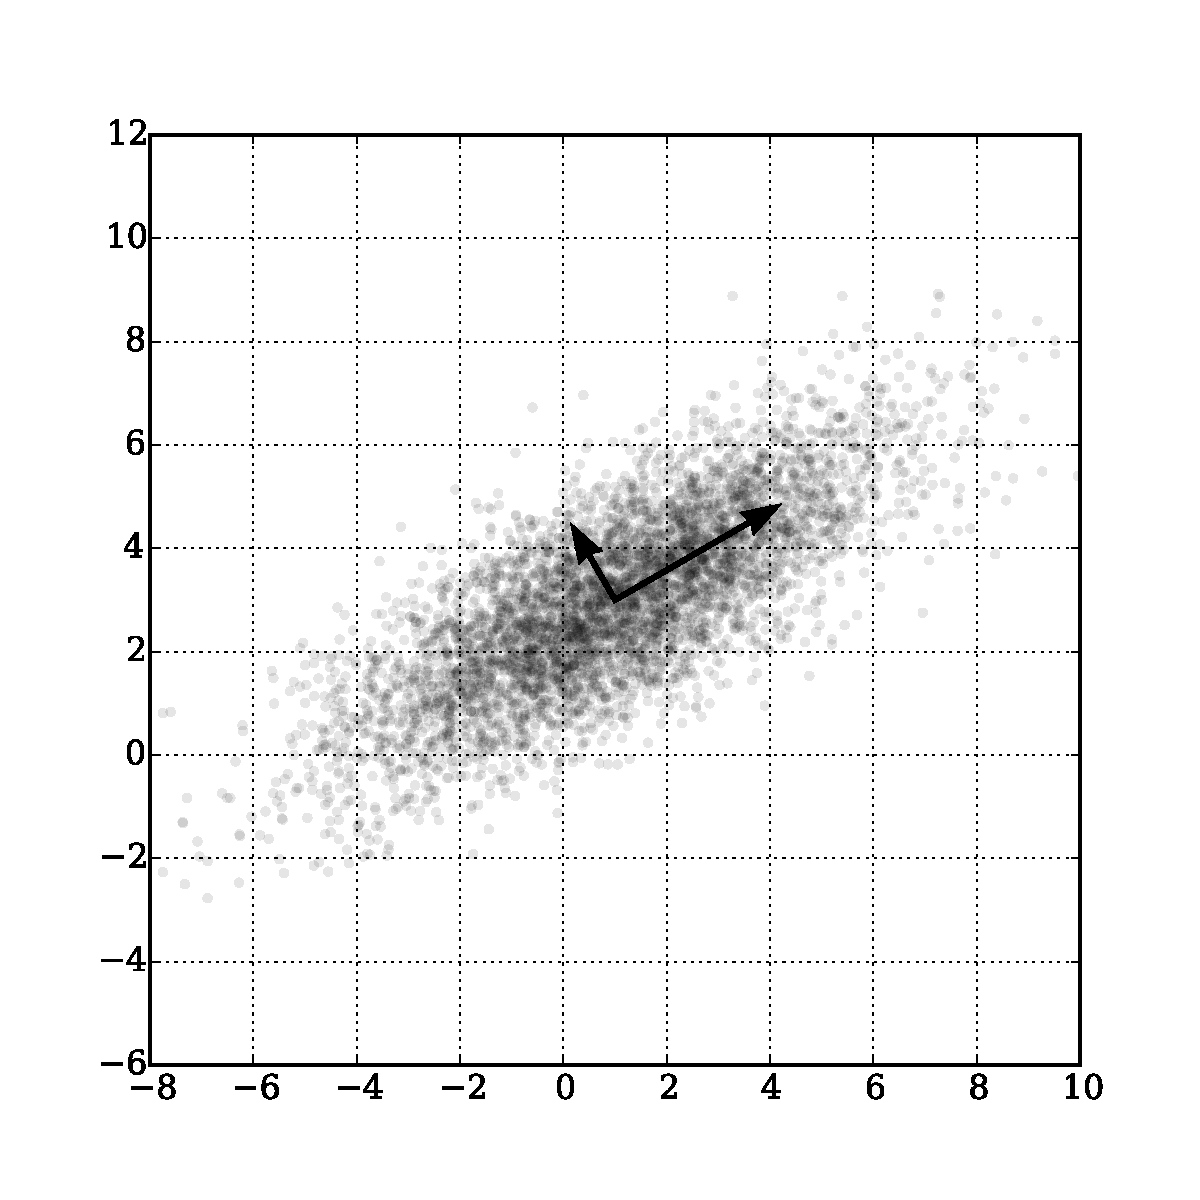
\includegraphics[width=\textwidth]{images/GaussianScatterPCA.pdf}\vspace{-3mm}
      {\tiny [Image from Wikimedia Commons]}}%
      \only<2->{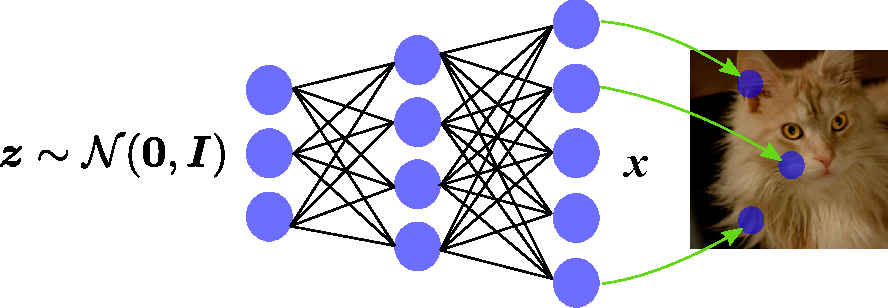
\includegraphics[width=\textwidth]{images/gen_model.pdf}}
   \end{column}
  \end{columns}
  \vspace{-8mm}
\end{frame}



%%%%%%%%%%%%%%%%%%%%%%%%%%%%%%%%%%%%%%%%%%%%%%%%%%%%%%%%%%%%%%
\begin{frame}{Formalising the generative model (I)}
  \begin{columns}
  \begin{column}{0.5\textwidth}
  The generative model:
 \begin{itemize}
  \item $\bs{z}\sim\mathcal{N}(\bs{0},\bs{I})$,
  \item $\bs{x}|\bs{z}\sim\MN(\bs{x};\bs{\mu}_{\bs{\theta}}(\bs{z}),\bs{\Sigma}_{\bs{\theta}}(\bs{z}))$,
 \end{itemize}
 where $\bs{\mu}_{\bs{\theta}}(\bs{z})$ and $\bs{\Sigma}_{\bs{\theta}}(\bs{z})$ will be implemented \textbf{by deep neural networks} parametrised by $\bs{\theta}$ with input $\bs{z}$.
   \end{column}
   \begin{column}{0.45\textwidth}
    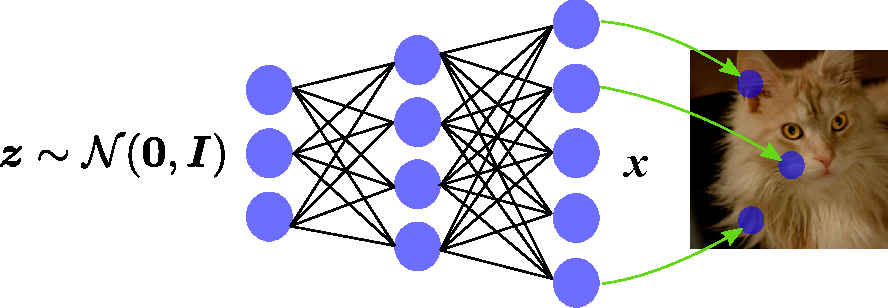
\includegraphics[width=\textwidth]{images/gen_model.pdf}
   \end{column}
  \end{columns}\vspace{5mm}

 \pause

 A few comments:
 \begin{enumerate}
 \item The optimal parameters $\bs{\theta}^*$ need to maximise the log-likelihood.
  %   We will be needing the posterior distribution $p(\bs{z}|\bs{x})$.
  \item $\bs{\theta}$ cannot be estimated in closed-form.
  \item $\bs{\mu}_{\bs{\theta}}(\bs{z})$ and $\bs{\Sigma}_{\bs{\theta}}(\bs{z})$ are differentiable w.r.t.\ $\bs{\theta}$, and $\bs{z}$.
  \item $\bs{\Sigma}_{\bs{\theta}}(\bs{z})$ needs to be a covariance matrix.
 \end{enumerate}

\end{frame}

%%%%%%%%%%%%%%%%%%%%%%%%%%%%%%%%%%%%%%%%%%%%%%%%%%%%%%%%%%%%%%
\begin{frame}{Formalising the generative model (II)}
  How can we ensure that $\bs{\Sigma}_{\bs{\theta}}(\bs{z})$ is a covariance matrix?
  \begin{itemize}
   \item The covariance matrix is assumed to be diagonal:
   \begin{equation}\bs{\Sigma}_{\bs{\theta}}(\bs{z}) = \left(\begin{array}{cccc}
   \nu^{(1)}_{\bs{\theta}}(\bs{z}) & 0 & \cdots & 0 \\
   0 & \nu^{(2)}_{\bs{\theta}}(\bs{z}) & \cdots & 0 \\
   \vdots & \vdots & \ddots & \vdots \\
   0 & 0 & \cdots & \nu^{(D)}_{\bs{\theta}}(\bs{z})
   \end{array}\right)\end{equation}
   Reduces complexity and memory, but also expressivity.
   \item We estimate the log-variance: $\eta^{(d)}_{\bs{\theta}}(\bs{z}) = \log \nu^{(d)}_{\bs{\theta}}(\bs{z})$:
   \begin{equation}\bs{\Sigma}_{\bs{\theta}}(\bs{z}) = \textrm{diag}_d \left(\exp \left(\eta^{(d)}_{\bs{\theta}}(\bs{z})\right)\right)\end{equation}
   The values of $\eta^{(d)}_{\bs{\theta}}(\bs{z})$ can be positive or negative.
  \end{itemize}


\end{frame}

%%%%%%%%%%%%%%%%%%%%%%%%%%%%%%%%%%%%%%%%%%%%%%%%%%%%%%%%%%%%%%
\begin{frame}{Formalising the generative model (III)}
  In terms of probabilistic dependencies, they are the same as PPCA:\vspace{3mm}\\
  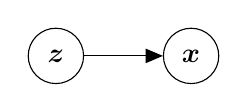
\begin{tikzpicture}[->]
   \node[latent,draw] (z)  {$\bs{z}$};
   \node[latent,draw,right=of z] (x) {$\bs{x}$};
   \edge{z} {x};
  \end{tikzpicture}\vspace{3mm}

  But I would like to draw also the non-lineariry:\vspace{3mm}

  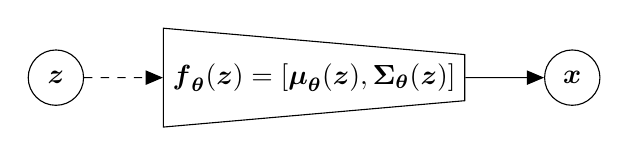
\begin{tikzpicture}[->]
   \node[latent,draw] (z)  {$\bs{z}$};
   \node[net,draw,trapezium angle=85,right=of z] (dec) {$\bs{f}_{\bs{\theta}}(\bs{z})=[\bs{\mu}_{\bs{\theta}}(\bs{z}),\bs{\Sigma}_{\bs{\theta}}(\bs{z})]$};
   \node[latent,draw,right=of dec] (x) {$\bs{x}$};
   \edge[dashed] {z} {dec};
   \edge{dec} {x};
  \end{tikzpicture}\vspace{3mm}

  The dependency of the parameters w.r.t.\ $\bs{z}$ is \textbf{deterministic}.\vspace{3mm}

  Denoted by $\bs{f}_{\bs{\theta}}(\bs{z}):\mathbb{R}^{d_z}\rightarrow\mathbb{R}^{2d_x}$, this non-linearity is implemented with a deep network, with parameters (weights and biases) $\bs{\theta}$.

\end{frame}

%%%%%%%%%%%%%%%%%%%%%%%%%%%%%%%%%%%%%%%%%%%%%%%%%%%%%%%%%%%%%%
\begin{frame}{The posterior distribution}
 For any EM-like procedure, we would need the posterior distribution:
 \begin{align}
  p(\bs{z}|\bs{x}) & \stackrel{(\bs{z})}{\propto}  p(\bs{x}|\bs{z})p(\bs{z}) \\
  &\stackrel{(\bs{z})}{\propto} \MN(\bs{x};\bs{\mu}_{\bs{\theta}}(\bs{z}),\bs{\Sigma}_{\bs{\theta}}(\bs{z})) \MN(\bs{z};\bs{0},\bs{I}) \\
  &\stackrel{(\bs{z})}{\propto} \frac{1}{|\bs{\Sigma}_{\bs{\theta}}(\bs{z})|^{1/2}} \exp\left(-\frac{1}{2} (\bs{x}-\bs{\mu}_{\bs{\theta}}(\bs{z}))^\top \bs{\Sigma}_{\bs{\theta}}^{-1}(\bs{z})(\bs{x}-\bs{\mu}_{\bs{\theta}}(\bs{z})) - \frac{1}{2}\lVert\bs{z}\rVert^2 \right)
 \end{align}\pause

 We cannot identify a distribution on $\bs{z}$.\vspace{3mm}

 The posterior distribution cannot be computed analytically!!!

\end{frame}

%%%%%%%%%%%%%%%%%%%%%%%%%%%%%%%%%%%%%%%%%%%%%%%%%%%%%%%%%%%%%%
\begin{frame}{Approximating the posterior distribution (I)}
 The posterior distribution needs to be approximated. We will propose a family of distributions, and find the \textbf{\textcolor{blue}{best candidate within this family}}.\vspace{3mm}\\

 \begin{figure}
  \centering
  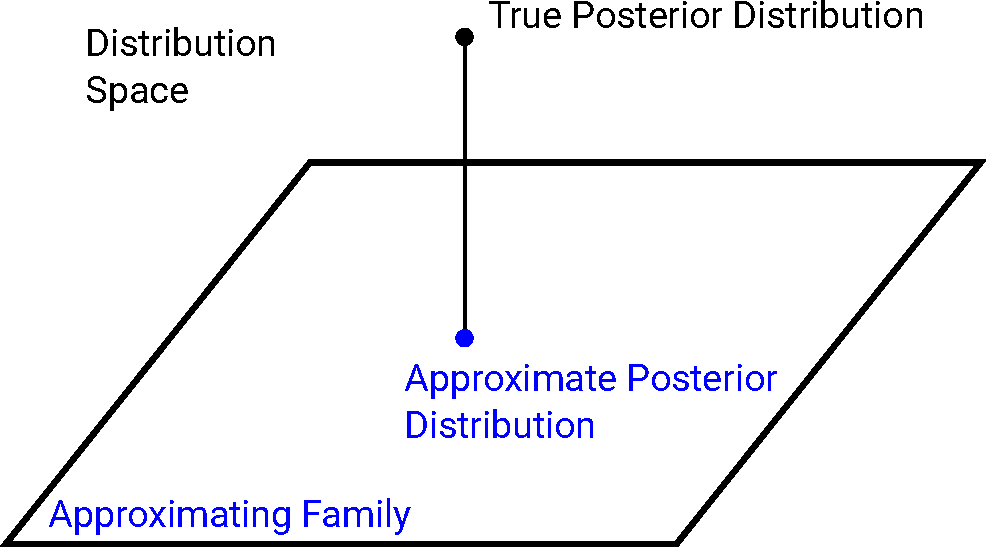
\includegraphics[width=0.6\textwidth]{images/distribution_projection.pdf}
 \end{figure}

\end{frame}

%%%%%%%%%%%%%%%%%%%%%%%%%%%%%%%%%%%%%%%%%%%%%%%%%%%%%%%%%%%%%%
\begin{frame}{Approximating the posterior distribution (II)}

 The posterior distribution will be approximated with \textbf{another} feed-forward network parametrised with $\bs{\phi}$:
 \begin{equation}p(\bs{z}|\bs{x})\approx q(\bs{z}|\bs{x}) = \MN(\bs{z};\tilde{\bs{\mu}}_{\bs{\phi}}(\bs{x}),\tilde{\bs{\Sigma}}_{\bs{\phi}}(\bs{x}))\end{equation}

 The approximating family is composed of all the distributions that can be expressed as above, for a certain value of $\bs{\phi}$.
 \begin{equation}\mathcal{G} = \{ \bs{g}_{\bs{\phi}}:\mathbb{R}^{d_x}\rightarrow\mathbb{R}^{2d_z};\bs{\phi}\in\bs{\Phi} \},\end{equation}
 with $\bs{g}_{\bs{\phi}}(\bs{x}) = [\tilde{\bs{\mu}}_{\bs{\phi}}(\bs{x}),\tilde{\bs{\Sigma}}_{\bs{\phi}}(\bs{x})]$.
\end{frame}

%%%%%%%%%%%%%%%%%%%%%%%%%%%%%%%%%%%%%%%%%%%%%%%%%%%%%%%%%%%%%%
\begin{frame}{Overall architecture}
 If we ``chain'' the posterior (encoder) and the generative (decoder) model:\vspace{3mm}
   \begin{figure}
    \centering
    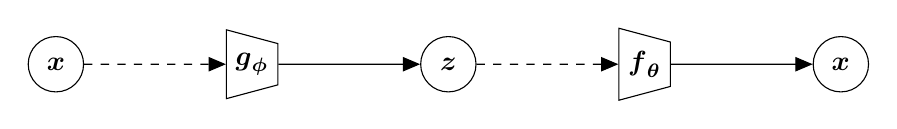
\begin{tikzpicture}[->]
    \node[latent,draw] (xi) {$\bs{x}$};
    \node[net,draw,right=1.8cm of xi] (enc) {$\bs{g}_{\bs{\phi}}$};
    \node[latent,draw,right=1.8cm of enc] (z)  {$\bs{z}$};
    \node[net,draw,right=1.8cm of z] (dec) {$\bs{f}_{\bs{\theta}}$};
    \node[latent,draw,right=1.8cm of dec] (x) {$\bs{x}$};
    \edge[dashed] {xi} {enc};
    \edge{enc} {z};
    \edge[dashed] {z} {dec};
    \edge{dec} {x};
    \end{tikzpicture}\\
    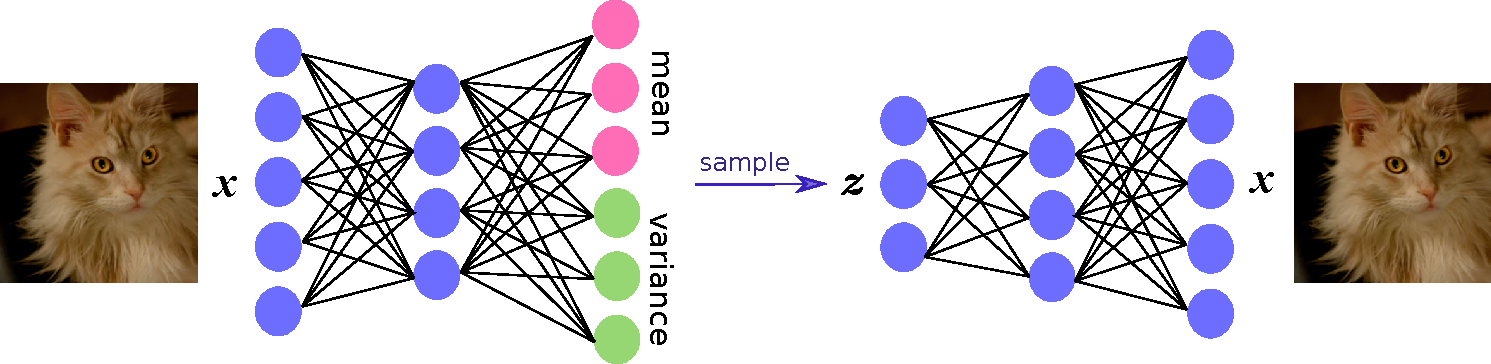
\includegraphics[width=0.8\textwidth]{images/geninf_model.pdf}
   \end{figure}
\begin{center}
 $ p(\bs{z}|\bs{x})\approx q(\bs{z}|\bs{x}) = \mathcal{N}\Big(\bs{z};\tilde{\bs{\mu}}_{\bs{\phi}}(\bs{x}),\tilde{\bs{\Sigma}}_{\bs{\phi}}(\bs{x})\Big) \qquad p_{\bs{\theta}}(\bs{x}|\bs{z}) =\mathcal{N}\Big(\bs{x};\bs{\mu}_{\bs{\theta}}(\bs{z}),\bs{\Sigma}_{\bs{\theta}}(\bs{z})\Big)$
\end{center}



%  This is why we call these architectures \textbf{variational autoencoders} VAE.\vspace{3mm}

 But how do we optimise for the parameters $\bs{\theta}$ and $\bs{\phi}$?

\end{frame}

%%%%%%%%%%%%%%%%%%%%%%%%%%%%%%%%%%%%%%%%%%%%%%%%%%%%%%%%%%%%%%
\begin{frame}{Learning - ELBO}
 If we recall the formulation for the EM:
 \begin{align*}
\log p(\bs{x}) &= \mathbb{E}_{q(\bs{z}|\bs{x})}\Big[\log \frac{p(\bs{x},\bs{z})}{q(\bs{z}|\bs{x})}\Big] + {\color{red} D_{\text{KL}}\Big(q(\bs{z}|\bs{x})\Big\lVert p(\bs{z}|\bs{x})\Big)}
\end{align*}\pause
Problem: the second term cannot be computed! But it's positive:
 \begin{align*}
\log p(\bs{x};\bs{\theta},\bs{\phi}) &\; {\color{red}\geq}\; {\color{blue} \mathbb{E}_{q_{\bs{\phi}}(\bs{z}|\bs{x})}\Big[\log \frac{p(\bs{x},\bs{z})}{q_{\bs{\phi}}(\bs{z}|\bs{x})}\Big]} \\
\log p(\bs{x};\bs{\theta},\bs{\phi}) &\; {\color{red}\geq}\; {\color{blue} \underbrace{\mathbb{E}_{q_{\bs{\phi}}(\bs{z}|\bs{x})}\Big[\log p_{\bs{\theta}}(\bs{x}|\bs{z})\Big]}_{\text{Reconstruction}} -  \underbrace{D_{\text{KL}}\Big(q_{\bs{\phi}}(\bs{z}|\bs{x})\Big\lVert p(\bs{z})\Big)}_{\text{Regularisation}}}
\end{align*}
This is known as \textbf{Evidence Lower-BOund or ELBO}: $\mathcal{L}_{\text{ELBO}}(\bs{\theta},\bs{\phi})$.\vspace{3mm}\\
Be VERY careful with these expressions: They look alike, but they are NOT the same.
\end{frame}

%%%%%%%%%%%%%%%%%%%%%%%%%%%%%%%%%%%%%%%%%%%%%%%%%%%%%%%%%%%%%%
\begin{frame}{Learning - Sampling}
 But we still have one problem:
 \begin{align*}
  \mathcal{L}_{\text{ELBO}}(\bs{\theta},\bs{\phi}) &= \underbrace{\mathbb{E}_{q_{\bs{\phi}}(\bs{z}|\bs{x})}\Big\{\log p_{\bs{\theta}}(\bs{x}|\bs{z})\Big\}}_{\text{Reconstruction}} -  \underbrace{D_{\text{KL}}\Big(q_{\bs{\phi}}(\bs{z}|\bs{x})\Big\lVert p(\bs{z})\Big)}_{\text{Regularisation}}
\end{align*}
To compute the ``reconstruction'' term we need to take the expectation w.r.t.\ $q_{\bs{\phi}}(\bs{z}|\bs{x})$, but recall that:
\begin{equation*}
  p_{\bs{\theta}}(\bs{x}|\bs{z}) = \mathcal{N}(\bs{x};\bs{\mu}_{\bs{\theta}}(\bs{z}),\bs{\Sigma}_{\bs{\theta}}(\bs{z})).
\end{equation*}
Due to the non-linearity, we cannot compute the reconstruction term in closed form\\ $\rightarrow$ we sample $R$ points $\hat{\bs{z}}^{(1)},\ldots,\hat{\bs{z}}^{(R)}$ from $q_{\bs{\phi}}$:
 \begin{align*}
  \mathcal{L}_{\text{ELBO}}(\bs{\theta},\bs{\phi}) &= \underbrace{\frac{1}{R}\sum_{r=1}^R\log p_{\bs{\theta}}(\bs{x}|\hat{\bs{z}}^{(r)})}_{\text{Reconstruction}} -  \underbrace{D_{\text{KL}}\Big(q_{\bs{\phi}}(\bs{z}|\bs{x})\Big\lVert p(\bs{z})\Big)}_{\text{Regularisation}}
\end{align*}
\end{frame}

%%%%%%%%%%%%%%%%%%%%%%%%%%%%%%%%%%%%%%%%%%%%%%%%%%%%%%%%%%%%%%
\begin{frame}{Learning - Gradient ascent?}
  Let's go back to the architecture:\vspace{-3mm}
\begin{figure}
  \centering
   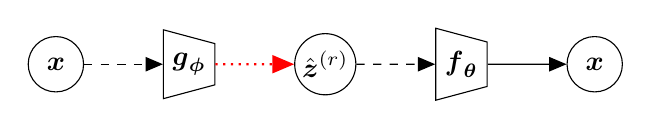
\begin{tikzpicture}[->]
   \node[latent,draw] (xi) {$\bs{x}$};
   \node[net,draw,right=of xi] (enc) {$\bs{g}_{\bs{\phi}}$};
   \node[latent,draw,right=of enc] (z)  {$\hat{\bs{z}}^{(r)}$};
   \node[net,draw,right=of z] (dec) {$\bs{f}_{\bs{\theta}}$};
   \node[latent,draw,right=of dec] (x) {$\bs{x}$};
   \edge[dashed] {xi} {enc};
   \edge[dotted,thick,red] {enc} {z};
   \edge[dashed] {z} {dec};
   \edge{dec} {x};
  \end{tikzpicture}
  \end{figure}\vspace{-3mm}

  Since there is no closed-form solution for the parameters (due to the non-linearity), we will learn the parameters using stochastic gradient ascent (to maximise the ELBO).\vspace{3mm}

  We assume that $\bs{g}_{\bs{\phi}}$ and $\bs{f}_{\bs{\theta}}$ are differentiable (we can compute the gradient).\vspace{3mm}

  The sampling operation ($\hat{\bs{z}}^{(r)}$) from $q_{\bs{\phi}}$ is {\color{red}NOT} differentiable w.r.t.\ $\bs{\phi}$.
\end{frame}

%%%%%%%%%%%%%%%%%%%%%%%%%%%%%%%%%%%%%%%%%%%%%%%%%%%%%%%%%%%%%%
\begin{frame}{Learning - Reparametrisation trick}
%  We use the so-called \textbf{reparametrisation trick}:\vspace{3mm}\\
  Instead of sampling directly from the posterior ($\hat{\bs{z}}^{(r)}\sim q_{\bs{\phi}}=\mathcal{N}(\tilde{\bs{\mu}}_{\bs{\phi}},\tilde{\bs{\Sigma}}_{\bs{\phi}})$) we sample as follows:
  \begin{equation*}
   \bar{\bs{z}}^{(r)} = \tilde{\bs{\Sigma}}_{\bs{\phi}}^{1/2} \bar{\bs{\epsilon}}^{(r)} + \tilde{\bs{\mu}}_{\bs{\phi}} \quad\text{with}\quad \bar{\bs{\epsilon}}^{(r)}\sim \mathcal{N}(\bs{0},\bs{I})
  \end{equation*}

  $\hat{\bs{z}}^{(r)}$ and $\bar{\bs{z}}^{(r)}$ follow the same distribution, BUT $\bar{\bs{z}}^{(r)}$ is differentiable w.r.t.\ $\bs{\phi}$!!!\vspace{3mm}\\\pause

  This is called the \textbf{reparametrisation trick} and can be used with other distributions.\vspace{-3mm}
  \begin{figure}
  \centering
    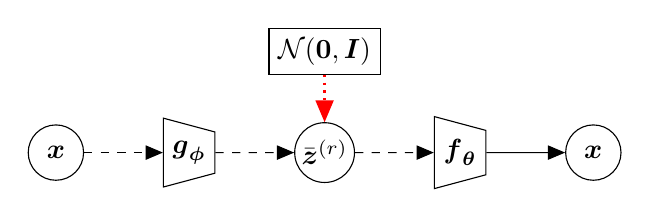
\begin{tikzpicture}[->]
   \node[latent,draw] (xi) {$\bs{x}$};
   \node[net,draw,right=of xi] (enc) {$\bs{g}_{\bs{\phi}}$};
   \node[latent,draw,right=of enc] (z)  {$\bar{\bs{z}}^{(r)}$};
   \node[net,draw,right=of z] (dec) {$\bs{f}_{\bs{\theta}}$};
   \node[latent,draw,right=of dec] (x) {$\bs{x}$};
   \node[draw,above=of z,yshift=-4mm] (standard) {$\mathcal{N}(\bs{0},\bs{I})$};
   \edge[dashed] {xi} {enc};
   \edge[dashed] {enc} {z};
   \edge[dotted,thick,red] {standard} {z};
   \edge[dashed] {z} {dec};
   \edge{dec} {x};
  \end{tikzpicture}
  \end{figure}\vspace{-3mm}
\end{frame}

%%%%%%%%%%%%%%%%%%%%%%%%%%%%%%%%%%%%%%%%%%%%%%%%%%%%%%%%%%%%%%
\begin{frame}{Learning - Reparametrisation trick (II)}
 \begin{figure}
  \centering
  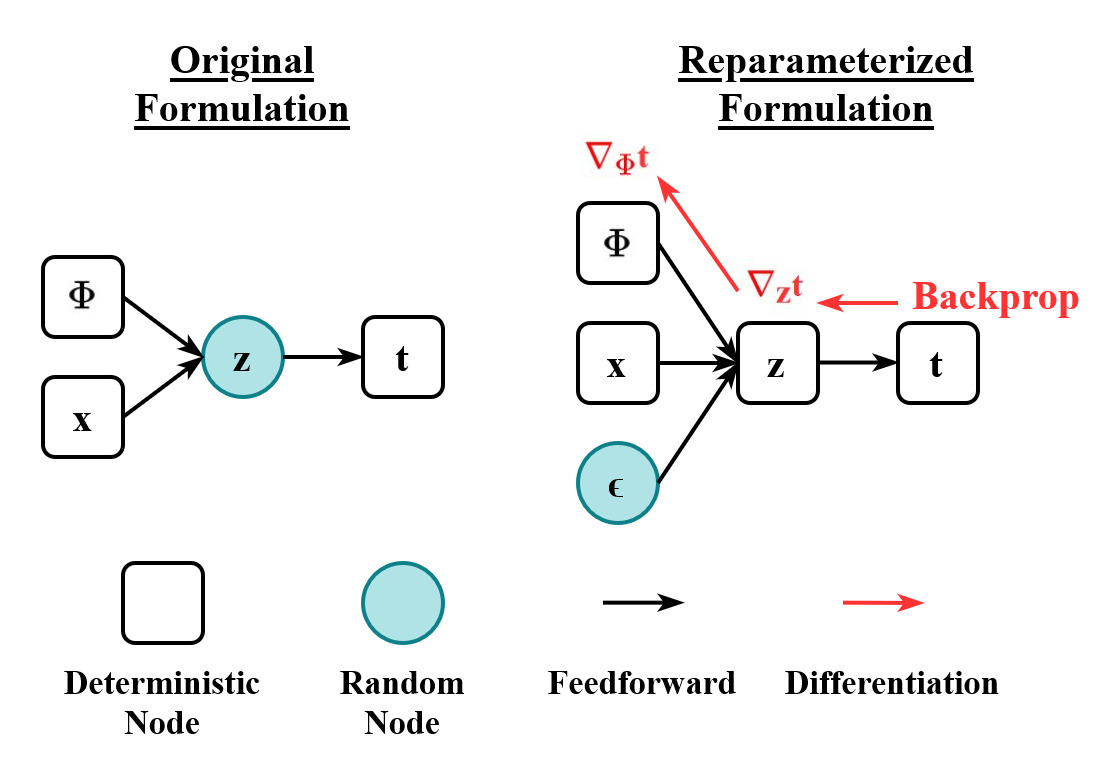
\includegraphics[width=0.5\textwidth]{images/ReparameterizationTrick.jpg}\vspace{-3mm}\\
  {\tiny [Image from Wikimedia Commons]}
 \end{figure}

\end{frame}

%%%%%%%%%%%%%%%%%%%%%%%%%%%%%%%%%%%%%%%%%%%%%%%%%%%%%%%%%%%%%%
\begin{frame}{Training VAE}

\begin{align*}
\log p(\bs{x}) &\geq \mathbb{E}_{q(\bs{z}|\bs{x})}\Big[\log \frac{p(\bs{x},\bs{z})}{q(\bs{z}|\bs{x})}\Big] = \mathcal{L}_{\text{ELBO}}(\bs{\theta},\bs{\phi})
\end{align*}

\begin{itemize}
\item One needs to sample from $q(\bs{z}|\bs{x})$ to compute the expectation.
\item This sampling needs the ``reparametrisation trick'' to be differentiable.
\item Most libraries solve a minimisation problem $\rightarrow$ we need to provide $-\mathcal{L}_{\text{ELBO}}(\bs{\theta},\bs{\phi})$.
\end{itemize}\vspace{3mm}

\pause

 \textbf{Posterior collapse}: common phenomenon when the posterior $q_{\bs{\phi}}$ gets to close to the standard prior. It can happen for various dimensions of $\bs{z}$ $\rightarrow$ the VAE stops learning.
 \begin{itemize}
  \item The KL term dominates the ELBO $\rightarrow$ weight the KL term with $\beta<1$.
  \item The data can be reduced to less dimensions than $D$ $\rightarrow$ decrease $D$.
 \end{itemize}
\end{frame}


%%%%%%%%%%%%%%%%%%%%%%%%%%%%%%%%%%%%%%%%%%%%%%%%%%%%%%%%%%%%%%%%%%%%%%%%%%%%
\begin{frame}{VAE: Summary}
\textbf{Generative model}. Prior:
	$p(\bs{z})=\mathcal{N}(\bs{z};\boldsymbol{0},\bs{I})$ and decoder: $p_{\bs{\theta}}(\bs{x}|\bs{z})=\mathcal{N}\Big(\bs{x};\bs{\mu}_{\bs{\theta}}(\bs{z}),\bs{\Sigma}_{\bs{\theta}}(\bs{z})\Big)$.

\textbf{Inference model} (encoder): $p_{\bs{\theta}}(\bs{z}|\bs{x}) \approx q_{\bs{\phi}}(\bs{z}|\bs{x})=\mathcal{N}\Big(\bs{z};\bs{\mu}_{\bs{\phi}}(\bs{x}),\bs{\Sigma}_{\bs{\phi}}(\bs{x})\Big)$
\begin{figure}
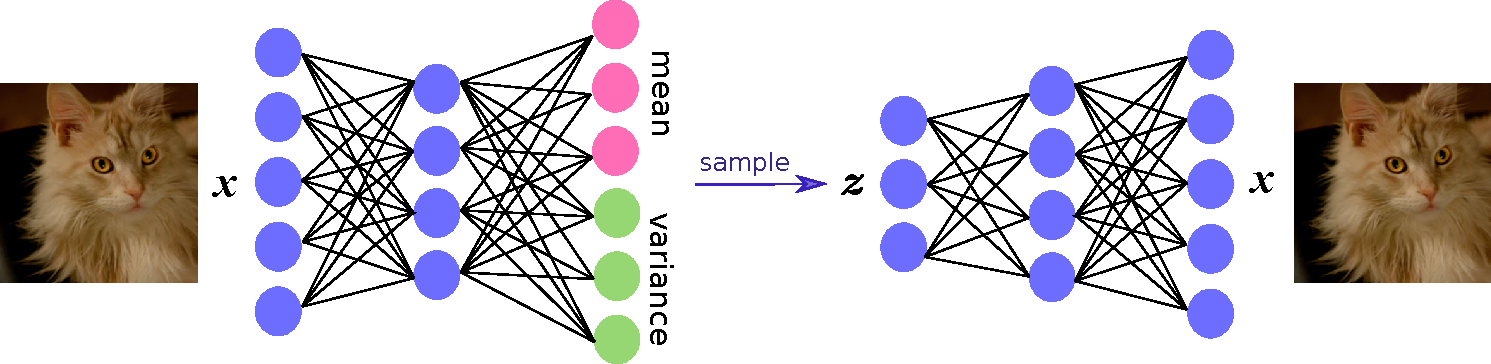
\includegraphics[scale=0.4]{images/geninf_model.pdf}
\end{figure}
\textbf{Training criterion} (maximise the evidence lower bound):
 \begin{align*}
  \mathcal{L}_{\text{ELBO}}(\bs{\theta},\bs{\phi}) &= \underbrace{\log p_{\bs{\theta}}(\bs{x}|\hat{\bs{z}})}_{\text{Reconstruction}} -  \underbrace{D_{\text{KL}}\Big(q_{\bs{\phi}}(\bs{z}|\bs{x})\Big\lVert p(\bs{z})\Big)}_{\text{Regularisation}}
\end{align*}
	where $\hat{\bs{z}}\sim q_{\bs{\phi}}$ is sampled using the reparametrisation trick.
\end{frame}

%%%%%%%%%%%%%%%%%%%%%%%%%%%%%%%%%%%%%%%%%%%%%%%%%%%%%%%%%%%%%%%%%%%%%%%%%%%%
\begin{frame}{ML with latent variables: EM vs VAE?}
ML with latent variable ($\bs{z}$) leads to EM\footnote{Dempster, A.P., \textit{et. al.}, (1977), Journal of the Royal Statistical Society.} and VI\footnote{Jordan, M. I., \textit{et. al.}, (1999),. Machine Learning.} build from {\footnotesize($\color{blue}q(\bs{z})$ is an arbitrary distribution)}:
\begin{align*}
\log p(\bs{x}) &= \underbrace{\mathbb{E}_{\color{blue}q(\bs{z})}\Big[\log \frac{p(\bs{x})p(\bs{z}|\bs{x})}{\color{blue}q(\bs{z})}\Big]}_{\text{M-step or VLB}} +  \underbrace{D_{\text{KL}}\Big({\color{blue}q(\bs{z})}\Big\lVert p(\bs{z}|\bs{x})\Big)}_{\text{E-step}}
\end{align*}
\begin{columns}
 \begin{column}{0.31\textwidth}
  \centering
  \underline{Exact EM}\\
  Simple $p(\bs{z}|\bs{x})$ \\
  ${\color{blue}q(\bs{z})}=p(\bs{z}|\bs{x})$\\
  Closed-form!\\
  $D_{\text{KL}} = 0$
 \end{column}
 \begin{column}{0.31\textwidth}

 \end{column}%
  \begin{column}{0.31\textwidth}
 \centering
  \underline{Variational AutoEncoder}\\
  $p(\bs{z}|\bs{x})$ ???\\
  ${\color{blue}q(\bs{z})} = q_{\bs{\phi}}(\bs{z})$\\
  $q_{\bs{\phi}}$ optimises ELBO/VLB\\
  $D_{\text{KL}}>0$ no closed form!
 \end{column}
\end{columns}
\end{frame}

%%%%%%%%%%%%%%%%%%%%%%%%%%%%%%%%%%%%%%%%%%%%%%%%%%%%%%%%%%%%%%%%%%%%%%%%%%%%
\begin{frame}{Mono-modal VAEs: the baselines}
\textbf{Audio-only}:\footnote{Leglaive, S., \textit{et. al.}, (2018), IEEE MLSP.}\vspace{-1mm}
\begin{columns}
 \begin{column}{0.5\textwidth}
 \resizebox{\textwidth}{!}{\input{tikz/a_vae.tex}}
%  \includegraphics[width=\textwidth]{images/a_vae_new.pdf}
 \end{column}
 \begin{column}{0.4\textwidth}
 \small
  $p_{\bs{\theta}}(\bs{\myos}_n | \bs{\mylz}_n)= \mathcal{N}_c\Big(\boldsymbol{0}, \text{diag}(\bs{\sigma}_{\myos}(\bs{\mylz}_n))\Big)$\\
  $q_{\bs{\phi}}(\bs{\mylz}_n|\bs{\myos}_n)= \mathcal{N}\Big(\bs{\mu}_{\bs{\mylz}}^a(\bs{\myos}_n), \text{diag}(\bs{\sigma}_{\bs{\mylz}}^a(\bs{\myos}_n))\Big)$
 \end{column}
\end{columns}
\pause
\textbf{Video-only}:
\vspace{-1mm}
\begin{columns}
 \begin{column}{0.5\textwidth}
  \resizebox{\textwidth}{!}{\renewcommand\drawNodes[2]{
  % #1 (str): namespace
  % #2 (list[list[str]]): list of labels to print in the node of each neuron
  \foreach \neurons [count=\lyrIdx] in #2 {
    \StrCount{\neurons}{,}[\lyrLength] % use xstring package to save each layer size into \lyrLength macro

    \ifthenelse{\equal{#1}{encoder}}{
        \ifnumequal{\lyrIdx}{1}
        {% True case
        \foreach \n [count=\nIdx] in \neurons
            \node[neuron,fill=green,fill opacity=0.2] (#1-\lyrIdx-\nIdx) at (0.7*\lyrIdx, \lyrLength/3.6-0.5*\nIdx) {\n};
        }
        {% False case
        \foreach \n [count=\nIdx] in \neurons
            \node[neuron] (#1-\lyrIdx-\nIdx) at (0.7*\lyrIdx, \lyrLength/3.6-0.5*\nIdx) {\n};
        }
    }{
        \ifnumequal{\lyrIdx}{2}
        {% True case
        \foreach \n [count=\nIdx] in \neurons
            \node[neuron,fill=green,fill opacity=0.2] (#1-\lyrIdx-\nIdx) at (0.7*\lyrIdx, \lyrLength/3.6-0.5*\nIdx) {\n};
        }
        {% False case
        \foreach \n [count=\nIdx] in \neurons
            \node[neuron] (#1-\lyrIdx-\nIdx) at (0.7*\lyrIdx, \lyrLength/3.6-0.5*\nIdx) {\n};
        }
    }
  }
}

\renewcommand\denselyConnectNodes[2]{
  % #1 (str): namespace
  % #2 (list[int]): number of nodes in each layer
  \foreach \n [count=\lyrIdx, remember=\lyrIdx as \previdx, remember=\n as \prevn] in #2 {
    \foreach \y in {1,...,\n} {
      \ifnum \lyrIdx > 1
        \foreach \x in {1,...,\prevn}
          \draw[-] (#1-\previdx-\x) -- (#1-\lyrIdx-\y);
      \fi
    }
  }
}

\begin{tikzpicture}[
    shorten >=1pt, shorten <=1pt,
    neuron/.style={circle, draw, minimum size=2ex, thick},
    legend/.style={font=\large\bfseries},
  ]

  % encoder
  \drawNodes{encoder}{{{,,,}, {,,}}}
  \denselyConnectNodes{encoder}{{4, 3}}

  % decoder
  \begin{scope}[xshift=3.7cm]
    \drawNodes{decoder}{{{,,}, {,,,}}}
    \denselyConnectNodes{decoder}{{3, 4}}
  \end{scope}
  
  \node[inner sep=0pt,left of=encoder-1-1,xshift=-0.5cm,yshift=-0.8cm] (input) {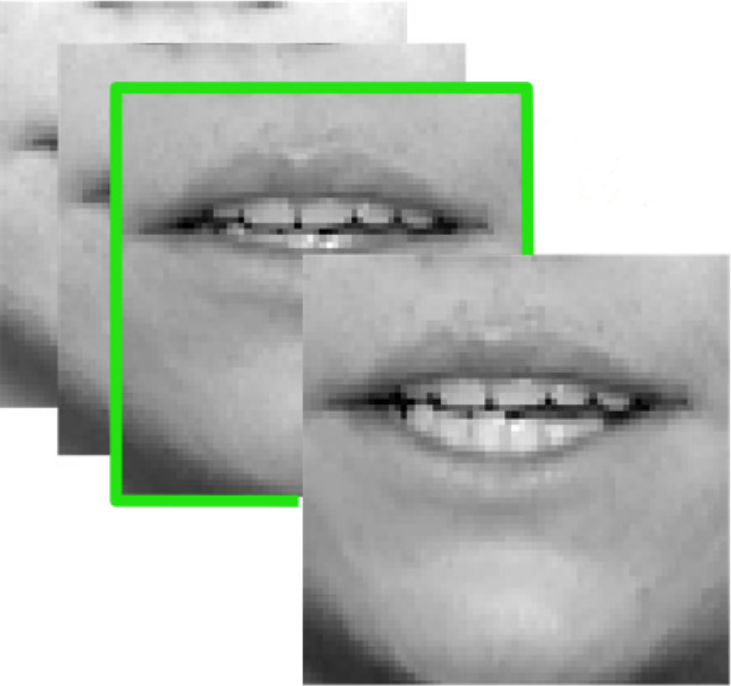
\includegraphics[width=.25\textwidth]{tikz/lips}};
  \node[inner sep=0pt,right of=decoder-2-1,xshift=0.5cm,yshift=-0.8cm] (output) {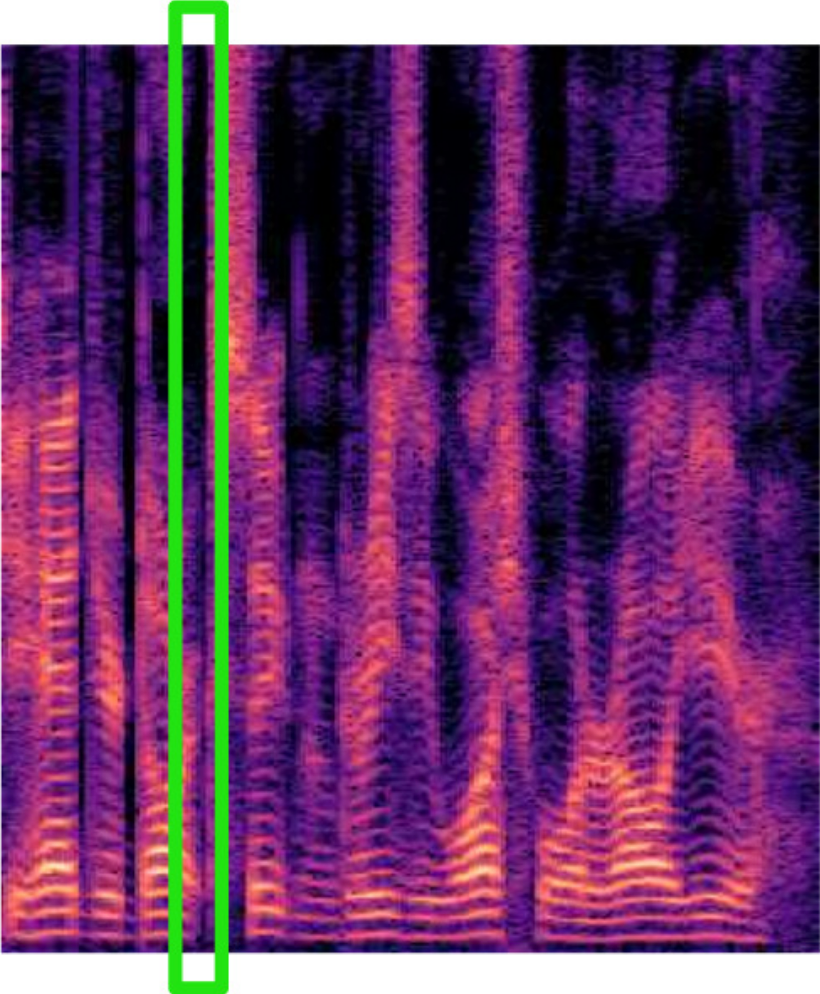
\includegraphics[width=.25\textwidth]{tikz/spectrogram}};
  
  % mu, sigma, sample nodes
  \foreach \idx in {1,...,3} {
      \coordinate[neuron, right=2 of encoder-2-2, xshift=-1.4cm, yshift=0.5*\idx cm-0.15cm, fill=red, fill opacity=0.2] (mu-\idx);
      \coordinate[neuron, right=2 of encoder-2-2, xshift=-1.4cm, yshift=-0.5*\idx cm+0.15cm, fill=red, fill opacity=0.2] (sigma-\idx);
      \coordinate[neuron, right=4 of encoder-2-2, xshift=-2.2cm, yshift=0.5*\idx cm-1cm, fill=red, fill opacity=0.2] (sample-\idx);
    }

  % mu, sigma, sample boxes
  \node [label={above right:$\bs{\mu}^v_{\bs{\mylz}}(\bs{\myov}_n)$}, fit=(mu-1) (mu-3), draw] (mu) {};
  \node [label={below right:$\bs{\sigma}^v_{\bs{\mylz}}(\bs{\myov}_n)$}, fit=(sigma-1) (sigma-3), draw] (sigma) {};
  \node [fit=(sample-1) (sample-3), draw] (sample) {};

  % mu, sigma, sample connections
  \draw[dashed] (mu.east) edge (sample.west) (sigma.east) -- (sample.west);
  \foreach \a in {1,2,3}
  \foreach \b in {1,2,3} {
      \draw[-] (encoder-2-\a) -- (mu-\b);
      \draw[-] (encoder-2-\a) -- (sigma-\b);
      \draw[-] (sample-\a) -- (decoder-1-\b);
    }

  % input + output labels
%   \foreach \idx in {1,...,4} {
%       \node[left=0 of encoder-1-\idx] {$x_\idx$};
%       \node[right=0 of decoder-2-\idx] {$\hat x_\idx$};
%     }
  \node[above=0.1 of encoder-1-1] {$\bs{\myov}_n$};
  \node[above=0.1 of decoder-2-1] {$\hat{\bs{\myos}}_n$};

\end{tikzpicture}
}
%   \includegraphics[width=\textwidth]{images/v_vae_new.pdf}
 \end{column}
 \begin{column}{0.4\textwidth}
 \small
  $p_{\bs{\theta}}(\bs{\myos}_n | \bs{\mylz}_n)= \mathcal{N}_c\Big(\boldsymbol{0}, \text{diag}(\bs{\sigma}_{\myos}(\bs{\mylz}_n))\Big)$\\
  $q_{\bs{\phi}}(\bs{\mylz}_n|\bs{\myov}_n)= \mathcal{N}\Big(\bs{\mu}_{\bs{\mylz}}^v(\bs{\myov}_n), \text{diag}(\bs{\sigma}_{\bs{\mylz}}^v(\bs{\myov}_n))\Big)$
 \end{column}
\end{columns}
\end{frame}

%%%%%%%%%%%%%%%%%%%%%%%%%%%%%%%%%%%%%%%%%%%%%%%%%%%%%%%%%%%%%%%%%%%%%%%%%%%%
\begin{frame}{Audio-visual Conditional VAE\footnote{Sadeghi, M., \textit{et. al.}, (2020), IEEE TASLP.}}
% VAE conditioned with visual frames:\vspace{2mm}
\begin{columns}
 \begin{column}{0.6\textwidth}
 \centering
%  Encoder-Decoder
   \resizebox{\textwidth}{!}{\renewcommand\drawNodes[2]{
  % #1 (str): namespace
  % #2 (list[list[str]]): list of labels to print in the node of each neuron
  \foreach \neurons [count=\lyrIdx] in #2 {
    \StrCount{\neurons}{,}[\lyrLength] % use xstring package to save each layer size into \lyrLength macro

    \ifthenelse{\equal{#1}{encoder}}{
        \ifnumequal{\lyrIdx}{1}
        {% True case
        \foreach \n [count=\nIdx] in \neurons
            \node[neuron,fill=green,fill opacity=0.2] (#1-\lyrIdx-\nIdx) at (0.7*\lyrIdx, \lyrLength/3.6-0.5*\nIdx) {\n};
        }
        {% False case
        \foreach \n [count=\nIdx] in \neurons
            \node[neuron] (#1-\lyrIdx-\nIdx) at (0.7*\lyrIdx, \lyrLength/3.6-0.5*\nIdx) {\n};
        }
    }{
        \ifnumequal{\lyrIdx}{2}
        {% True case
        \foreach \n [count=\nIdx] in \neurons
            \node[neuron,fill=green,fill opacity=0.2] (#1-\lyrIdx-\nIdx) at (0.7*\lyrIdx, \lyrLength/3.6-0.5*\nIdx) {\n};
        }
        {% False case
        \foreach \n [count=\nIdx] in \neurons
            \node[neuron] (#1-\lyrIdx-\nIdx) at (0.7*\lyrIdx, \lyrLength/3.6-0.5*\nIdx) {\n};
        }
    }
  }
}

\renewcommand\denselyConnectNodes[2]{
  % #1 (str): namespace
  % #2 (list[int]): number of nodes in each layer
  \foreach \n [count=\lyrIdx, remember=\lyrIdx as \previdx, remember=\n as \prevn] in #2 {
    \foreach \y in {1,...,\n} {
      \ifnum \lyrIdx > 1
        \foreach \x in {1,...,\prevn}
          \draw[-] (#1-\previdx-\x) -- (#1-\lyrIdx-\y);
      \fi
    }
  }
}

\begin{tikzpicture}[
    shorten >=1pt, shorten <=1pt,
    neuron/.style={circle, draw, minimum size=2ex, thick},
    legend/.style={font=\large\bfseries},
  ]

  % encoder
  \drawNodes{encoder}{{{,,,,,}, {,,}}}
  \denselyConnectNodes{encoder}{{6, 3}}

  % decoder
  \begin{scope}[xshift=3.7cm]
    \drawNodes{decoder}{{{,,}, {,,,}}}
    \denselyConnectNodes{decoder}{{3, 4}}
  \end{scope}
  
  \node[inner sep=0pt,left of=encoder-1-1,xshift=-0.5cm,yshift=-0.2cm] (input) {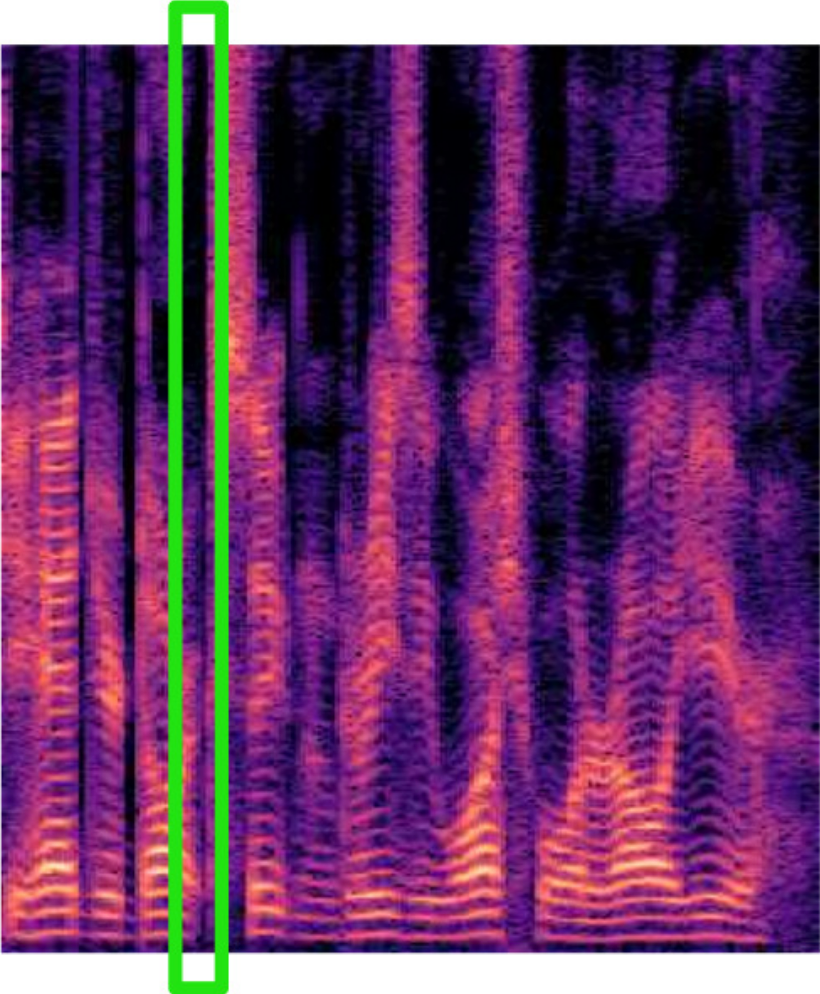
\includegraphics[width=.25\textwidth]{tikz/spectrogram}};
  \node[inner sep=0pt,left of=encoder-1-1,xshift=-0.5cm,yshift=-2.4cm] (input2) {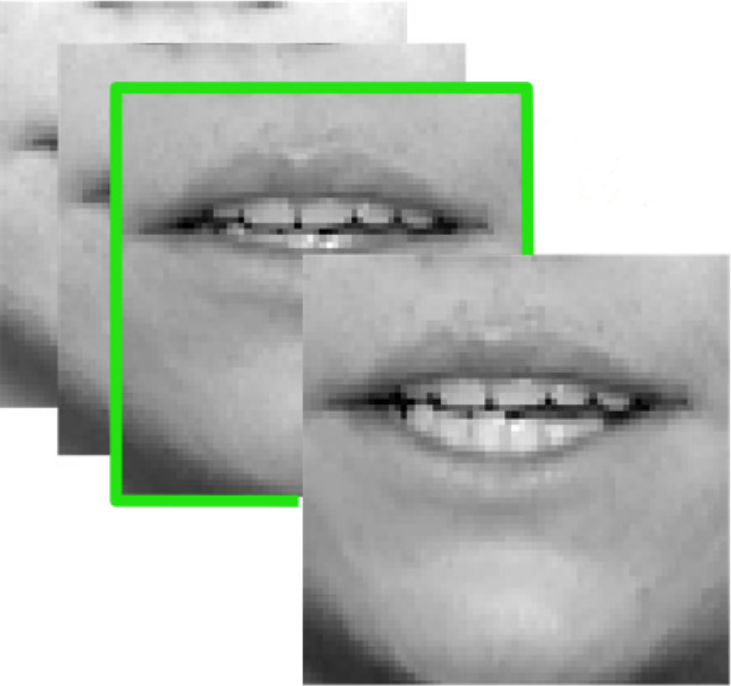
\includegraphics[width=.25\textwidth]{tikz/lips}};
  \node[inner sep=0pt,right of=decoder-2-1,xshift=0.5cm,yshift=-0.8cm] (output) {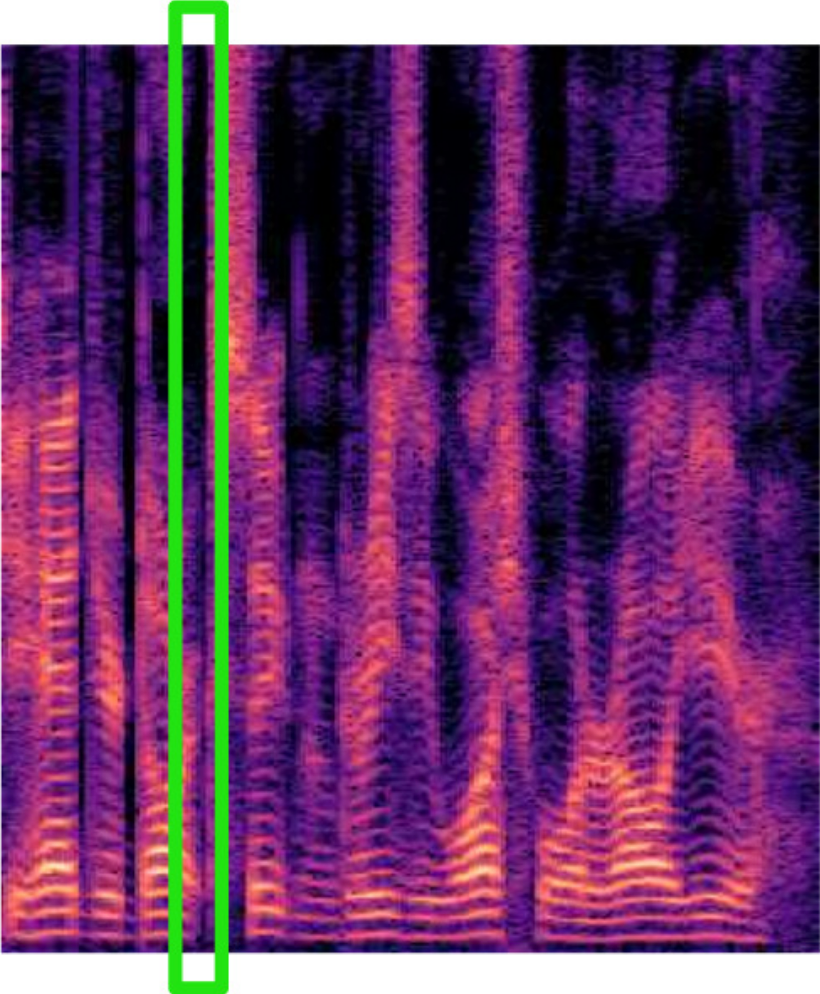
\includegraphics[width=.25\textwidth]{tikz/spectrogram}};
  
  % mu, sigma, sample nodes, conditioning
  \foreach \idx in {1,...,3} {
      \coordinate[neuron, right=2 of encoder-2-2, xshift=-1.4cm, yshift=0.5*\idx cm-0.15cm, fill=red, fill opacity=0.2] (mu-\idx);
      \coordinate[neuron, right=2 of encoder-2-2, xshift=-1.4cm, yshift=-0.5*\idx cm+0.15cm, fill=red, fill opacity=0.2] (sigma-\idx);
      \coordinate[neuron, right=4 of encoder-2-2, xshift=-2.2cm, yshift=0.5*\idx cm-.15cm, fill=red, fill opacity=0.2] (sample-\idx);
      \coordinate[neuron, right=4 of encoder-2-2, xshift=-2.2cm, yshift=0.5*\idx cm-1.85cm, fill=green, fill opacity=0.2] (cond-\idx);
    }
    
  \node[inner sep=0pt,below of=cond-1,xshift=0.2cm,yshift=0.2cm] (cond) {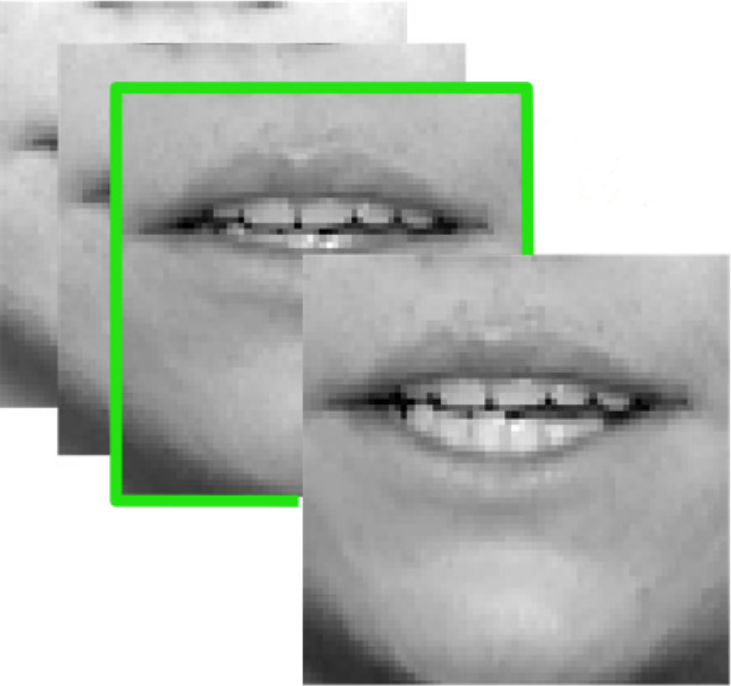
\includegraphics[width=.1\textwidth]{tikz/lips}};

  % mu, sigma, sample boxes
  \node [label={above:$\bs{\mu}^{av}_{\bs{\mylz}}(\bs{\myos}_n,\bs{\myov}_n)$}, fit=(mu-1) (mu-3), draw] (mu) {};
  \node [label={below:$\bs{\sigma}^{av}_{\bs{\mylz}}(\bs{\myos}_n,\bs{\myov}_n)$}, fit=(sigma-1) (sigma-3), draw] (sigma) {};
  \node [fit=(sample-1) (sample-3), draw] (sample) {};

  % mu, sigma, sample connections
  \draw[dashed] (mu.east) edge (sample.west) (sigma.east) -- (sample.west);
  \foreach \a in {1,2,3}
  \foreach \b in {1,2,3} {
      \draw[-] (encoder-2-\a) -- (mu-\b);
      \draw[-] (encoder-2-\a) -- (sigma-\b);
      \draw[-] (sample-\a) -- (decoder-1-\b);
      \draw[-] (cond-\a) -- (decoder-1-\b);
    }

  % input + output labels
%   \foreach \idx in {1,...,4} {
%       \node[left=0 of encoder-1-\idx] {$x_\idx$};
%       \node[right=0 of decoder-2-\idx] {$\hat x_\idx$};
%     }
  \node[above=0.1 of encoder-1-1] {$\bs{\myos}_n$};
  \node[below=0.1 of encoder-1-6] {$\bs{\myov}_n$};
  \node[above=0.1 of decoder-2-1] {$\hat{\bs{\myos}}_n$};

\end{tikzpicture}
}\vspace{2mm}
%   \includegraphics[width=\textwidth]{images/av_vae_new.pdf}
{\small
  $p_{\bs{\theta}}(\bs{\myos}_n | \bs{\mylz}_n,\bs{\myov}_n)= \mathcal{N}_c\Big(\boldsymbol{0}, \text{diag}(\bs{\sigma}_{\myos}(\bs{\mylz}_n,\bs{\myov}_n))\Big)$\vspace{3mm}\\
  $q_{\bs{\phi}}(\bs{\mylz}_n|\bs{\myov}_n,\bs{\myos}_n)= \mathcal{N}\Big(\bs{\mu}_{\bs{\mylz}}^{av}(\bs{\myov}_n,\bs{\myos}_n), \text{diag}(\bs{\sigma}_{\bs{\mylz}}^{av}(\bs{\myov}_n,\bs{\myos}_n))\Big)$}
 \end{column}
 \begin{column}{0.4\textwidth}
 \centering
 \only<2-3>{\alert{\Large What will this learn?}\vspace{2mm}\\}
 \only<3>{\Large To ignore the video!}
\only<4>{Visual Prior
 \resizebox{\textwidth}{!}{\input{tikz/v_prior_vae.tex}}
% \includegraphics[width=\textwidth]{images/prior_av_vae.pdf}
 {\small
  $p_{\bs{\theta}}(\bs{\mylz}_n|\bs{\myov}_n)= \mathcal{N}\Big(\bs{\mu}_{\bs{\mylz}}^v(\bs{\myov}_n), \text{diag}(\bs{\sigma}_{\bs{\mylz}}^v(\bs{\myov}_n))\Big)$}}
 \end{column}
\end{columns}
\end{frame}

%%%%%%%%%%%%%%%%%%%%%%%%%%%%%%%%%%%%%%%%%%%%%%%%%%%%%%%%%%%%%%%%%%%%%%%%%%%%
\begin{frame}{Learning AV Conditional VAE}
 On top of adding a video-only prior, we optimize a modified ELBO:
\begin{align*}
\hspace{-5mm}\mathcal{L}\left(\bs{\theta}, \bs{\phi} \right) =\sum_{n}  &{\alert{(1-\alpha)}}\Big(\E_{q_{\bs{\phi}}(\bs{z}_n|\bs{s}_n,\bs{v}_n;)}\Big[ \ln p_{\bs{\theta}}\left(\bs{s}_n | \bs{z}_n,\bs{v}_n \right) \Big]-D_{\text{KL}}\Big(q_{\bs{\phi}}\left(\bs{z}_n | \bs{s}_n,\bs{v}_n \right) \parallel p_{\bs{\theta}}(\bs{z}_n| \bs{v}_n)\Big)\Big)\\
\hspace{-5mm}& {+\alert{\alpha\,\E_{p_{\bs{\theta}}(\bs{z}_n| \bs{v}_n)}\Big[ \ln p_{\bs{\theta}}\left(\bs{s}_n | \bs{z}_n,\bs{v}_n \right) \Big]}}
\end{align*}

{$\Rightarrow \alpha>0 $ gives some reconstruction power to the visual prior!}\vspace{4mm}

{This provides the parameters of the clean speech model $\bs{\theta}$.}

\end{frame}

%%%%%%%%%%%%%%%%%%%%%%%%%%%%%%%%%%%%%%%%%%%%%%%%%%%%%%%%%%%%%%%%%%%%%%%%%%%
\begin{frame}{AV Conditional VAE for Speech Enhancement}
\begin{figure}
\centering
\only<1>{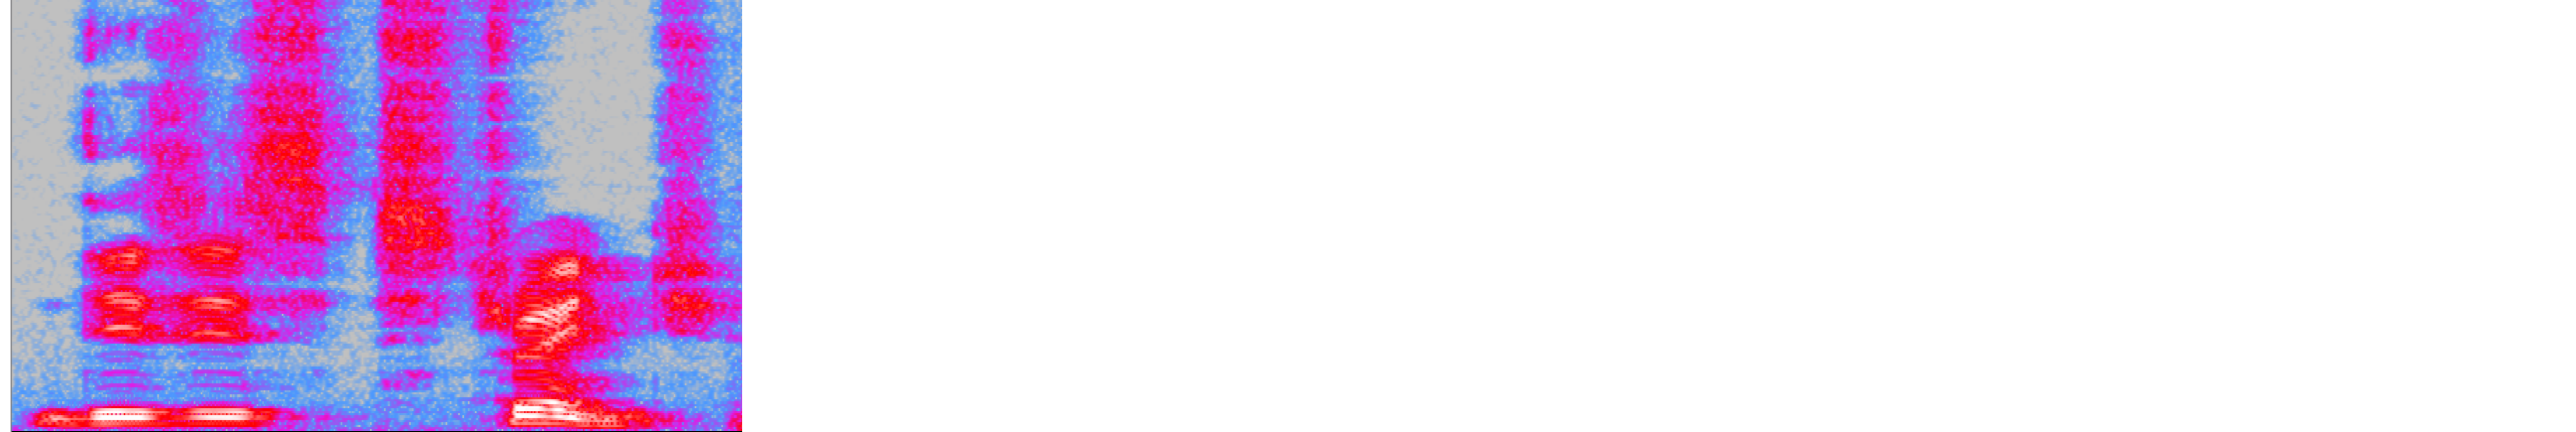
\includegraphics[width=0.8\textwidth]{images/spectrogram_cut.png}}%
\only<2->{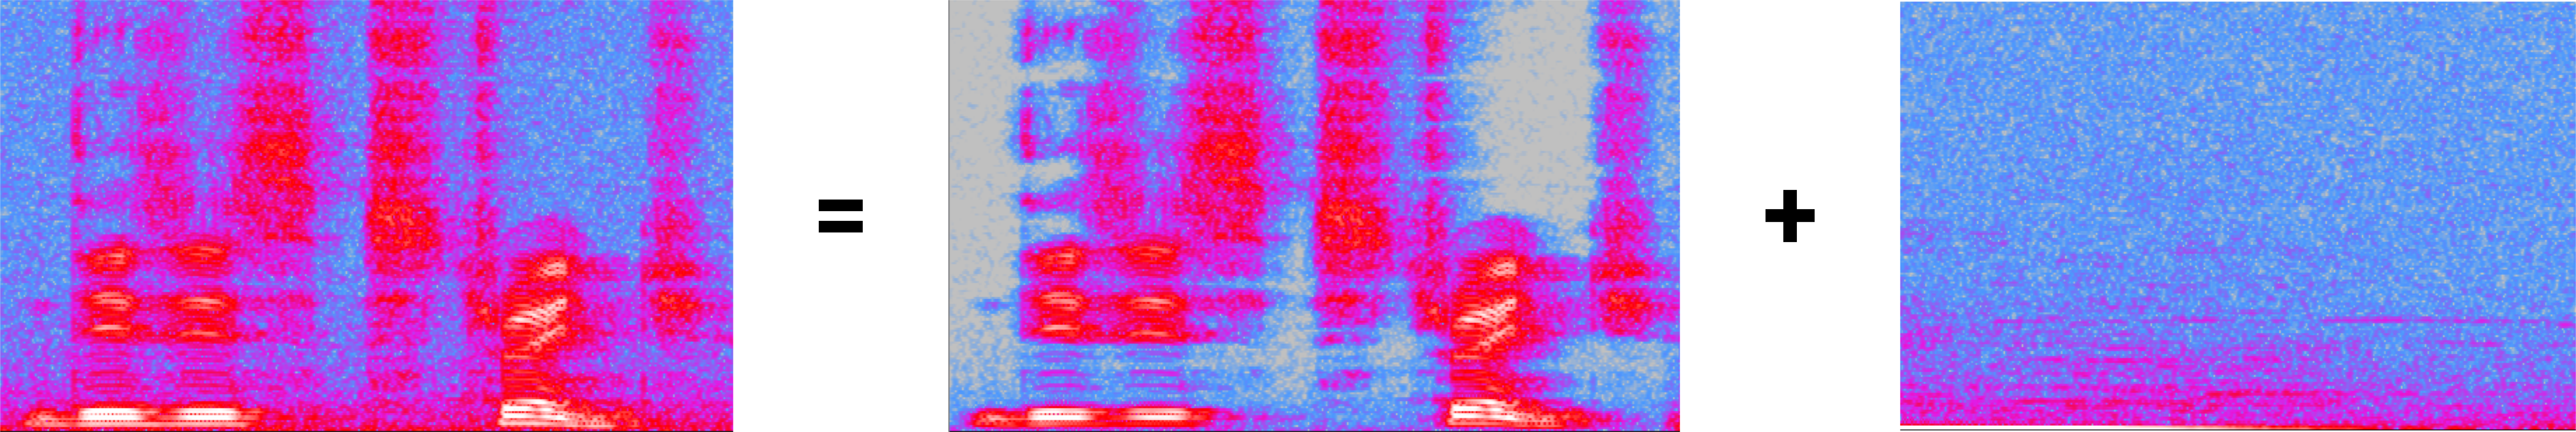
\includegraphics[width=0.8\textwidth]{images/spectrogram.png}}
\end{figure}
\vspace{-3mm}
\begin{equation*}
\only<1>{{\color{green}\underbrace{\mathbf{s}}_{\text{Clean speech}}} {\color{white}\quad\qquad+\quad\qquad \underbrace{\mathbf{b}}_{\text{Noise signal}}  \quad\qquad=\quad\qquad {\underbrace{\mathbf{x}}_{\text{Noisy mixture}}}}}
\only<2->{{\color{green}\underbrace{\mathbf{x}}_{\text{Noisy mixture}}}\quad\quad = \quad\quad {\color{red}\underbrace{\mathbf{s}}_{\text{Clean speech}}} \quad\qquad+\quad\qquad {\color{gray}\underbrace{\mathbf{b}}_{\text{Noise signal}}} }
\end{equation*}

\begin{columns}
 \begin{column}{0.5\textwidth}
  \only<1-2>{\alert<1>{\textbf{Train}} -- Model for \textcolor<1>{green}{clean data}: $\{{\only<1>{\color{green}}\bs{s}_i}\}_{i=1}^N$.
    \begin{center}
    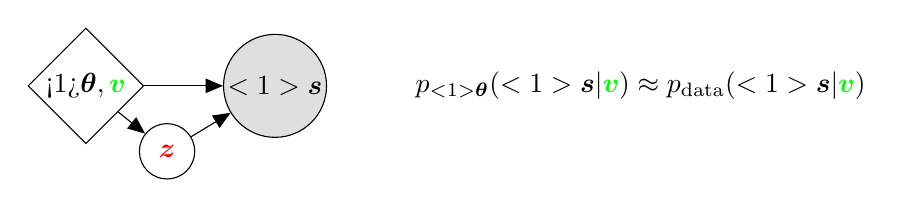
\begin{tikzpicture}
            \node[det] (theta) {\alert<1>{$\bs{\theta},\bs{\myov}$}};
            \node[latent,below right=of theta,xshift=-3mm,yshift=5mm] (z) {$\bs{\mylz}$};
            \node[obs,right=of theta] (s) {$\only<1>{\color{green}}\bs{s}$};
            \node[right=of s] (disc) {$p_{\alert<1>{\bs{\theta}}}({\only<1>{\color{green}}\bs{s}}|\bs{\myov})\approx p_{\text{data}}({\only<1>{\color{green}}\bs{s}}|\bs{\myov})$};
            \edge{theta} {s};
            \edge{theta} {z}; \edge{z} {s};
    \end{tikzpicture}
    \end{center}
    Then freeze $\alert<1>{\bs{\theta}}$ at test/adaptation time.}%
      \only<3>{Learn the parameters of the noise with a (slightly more complex) EM algorithm: E-step compute posterior of $\bs{\myls},\bs{\mylz}$, M-step update $\alert{\bs{\psi}}$.\vspace{4mm}\\
      Compute the most likely speech signal {\color{red}$\hat{\bs{s}}$}.}
 \end{column}\pause
 \begin{column}{0.5\textwidth}
  \textbf{Test} -- learn the \alert{noise parameters} from {\color{green} noisy samples $\mathbf{x}$} and estimate the {\color{red} clean speech $\hat{\bs{s}}$}:
    \begin{center}
    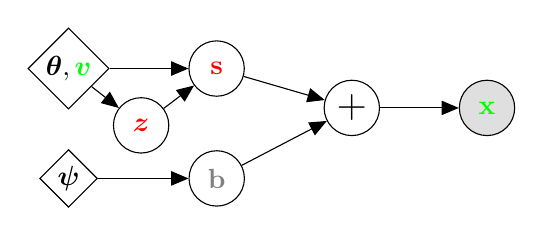
\begin{tikzpicture}
            \node[det] (theta) {$\bs{\theta},\bs{\myov}$};
            \node[latent,below right=of theta,xshift=-3mm,yshift=5mm] (z) {$\bs{\mylz}$};
            \node[latent,right=of theta] (s) {$\color{red}\mathbf{s}$};
            \node[det,below=of theta,yshift=5mm] (eta) {$\alert{\bs{\psi}}$};
            \node[latent,right=of eta,xshift=1.5mm] (b) {$\color{gray}\mathbf{b}$};
            \node[latent,right=of s,yshift=-5mm] (plus) {\Large$+$};
            \node[obs,right=of plus] (x) {$\color{green}\mathbf{x}$};
            \edge{theta} {s};
            \edge{eta} {b};
            \edge{s,b} {plus};
            \edge{plus} {x};
            \edge{theta} {z}; \edge{z} {s};
    \end{tikzpicture}
    \end{center}
 \end{column}%
\end{columns}

% \textbf{Note}: at test time, $\bs{\theta}$ is frozen, and $\mathbf{s}$ becomes a latent variable.
\end{frame}



%%%%%%%%%%%%%%%%%%%%%%%%%%%%%%%%%%%%%%%%%%%%%%%%%%%%%%%%%%%%%%%%%%%%%%%%%%%
\begin{frame}{AV Conditional VAE for Speech Enhancement}
\begin{figure}
\centering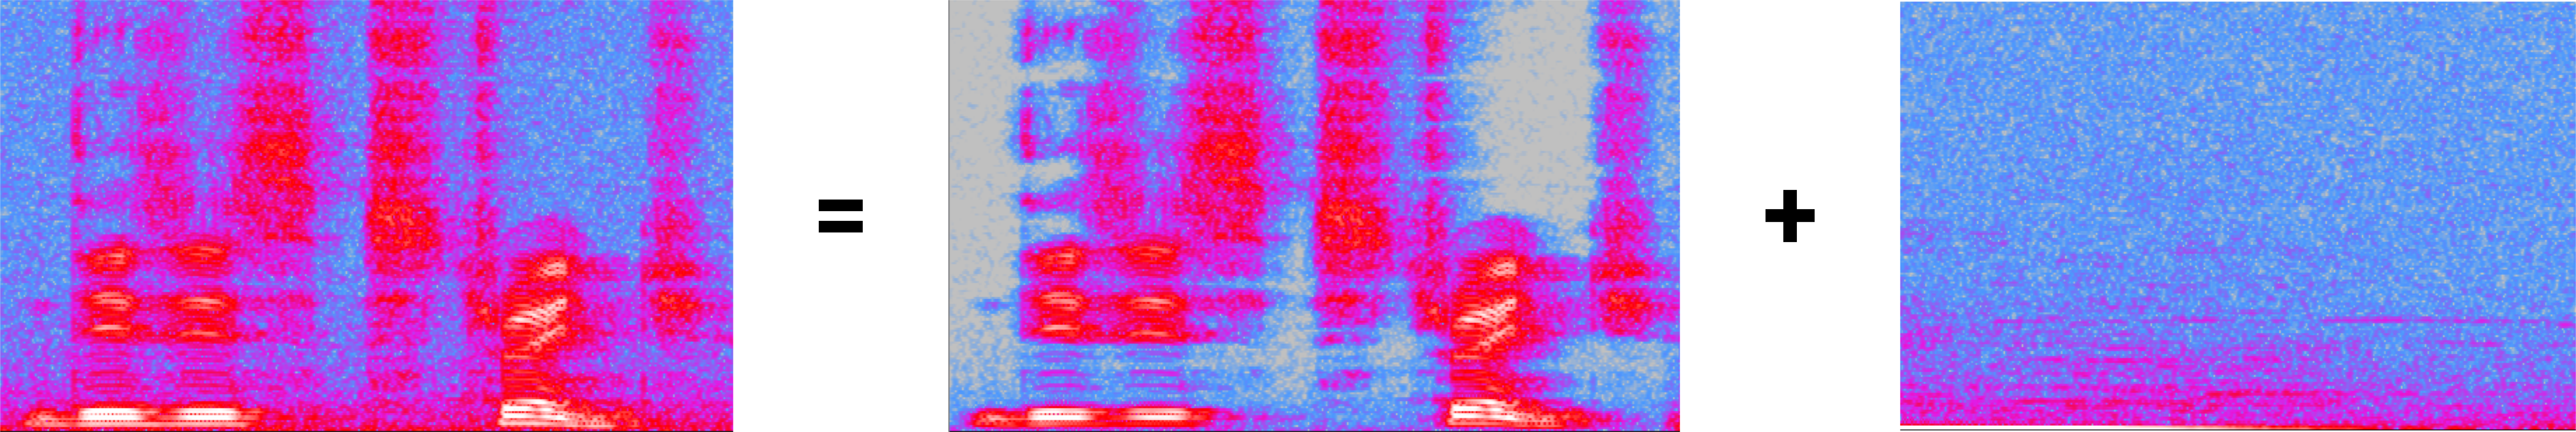
\includegraphics[width=0.8\textwidth]{images/spectrogram.png}
\end{figure}
\vspace{-3mm}
\begin{equation*}
{\color{green}\underbrace{\mathbf{x}}_{\text{Noisy mixture}}}\quad\quad = \quad\quad {\color{red}\underbrace{\mathbf{s}}_{\text{Clean speech}}} \quad\qquad+\quad\qquad {\color{gray}\underbrace{\mathbf{b}}_{\text{Noise signal}}}
\end{equation*}

\begin{columns}
 \begin{column}{0.4\textwidth}
  Minimize MSE $\rightarrow$ Wiener Filter\\
  {\footnotesize (signal and noise power are perfectly known)}
 \begin{equation*}
   {\color{red}\hat{\bs{s}}} = \frac{\color{red}{\bs{\sigma}_{\bs{s}}}}{{\color{red}{\bs{\sigma}_{\bs{s}}}} + \color{gray}{\bs{\sigma}_{\bs{b}}}} {\color{green}\bs{x}}
 \end{equation*}
 \end{column}\pause
 \begin{column}{0.4\textwidth}
 VAE-based Wiener Filter
  \[\hat{\bs{\myls}}_{n} = \left(\frac{1}{R}\sum_{r=1}^R  \frac{ \bs{\sigma}_{\myls}(\mathbf{\mylz}^{(r)},\bs{\myov}_n)}{\bs{\sigma}_{\myls}(\mathbf{\mylz}^{(r)},\bs{\myov}_n) + \alert{\boldsymbol{\psi}}^\ast_n}\right) \bs{\myox}_{n}.\]
 \end{column}%
\end{columns}

% \textbf{Note}: at test time, $\bs{\theta}$ is frozen, and $\mathbf{s}$ becomes a latent variable.
\end{frame}


\begin{frame}{Limitations}
\begin{itemize}
 \item This method systematically fuses auditory and visual data.
 \item Both data types must always be available and clean.
\end{itemize}
Not convenient in many situations:
\begin{center}
	\begin{figure}
		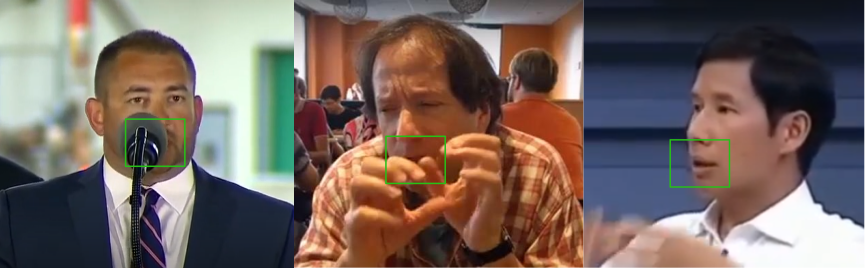
\includegraphics[scale=0.3]{images/drawing.png}
	\end{figure}
\end{center}
\end{frame}



%%%%%%%%%%%%%%%%%%%%%%%%%%%%%%%%%%%%%%%%%%%%%%%%%%%%%%%%%%%%%%%%%%%%%%%%%%%%
\begin{frame}{VAE Mixture Model\footnote{Sadeghi, M., \textit{et. al.}, (2021), IEEE ICASSP.}}
  \begin{columns}
 \centering
  \begin{column}{0.6\textwidth}
    \resizebox{\textwidth}{!}{\renewcommand\drawNodes[2]{
  % #1 (str): namespace
  % #2 (list[list[str]]): list of labels to print in the node of each neuron
  \foreach \neurons [count=\lyrIdx] in #2 {
    \StrCount{\neurons}{,}[\lyrLength] % use xstring package to save each layer size into \lyrLength macro

    \ifthenelse{\equal{#1}{encoder}}{
        \ifnumequal{\lyrIdx}{1}
        {% True case
        \foreach \n [count=\nIdx] in \neurons
            \node[neuron,fill=green,fill opacity=0.2] (#1-\lyrIdx-\nIdx) at (0.7*\lyrIdx, \lyrLength/3.6-0.5*\nIdx) {\n};
        }
        {% False case
        \foreach \n [count=\nIdx] in \neurons
            \node[neuron] (#1-\lyrIdx-\nIdx) at (0.7*\lyrIdx, \lyrLength/3.6-0.5*\nIdx) {\n};
        }
    }{
        \ifnumequal{\lyrIdx}{2}
        {% True case
        \foreach \n [count=\nIdx] in \neurons
            \node[neuron,fill=green,fill opacity=0.2] (#1-\lyrIdx-\nIdx) at (0.7*\lyrIdx, \lyrLength/3.6-0.5*\nIdx) {\n};
        }
        {% False case
        \foreach \n [count=\nIdx] in \neurons
            \node[neuron] (#1-\lyrIdx-\nIdx) at (0.7*\lyrIdx, \lyrLength/3.6-0.5*\nIdx) {\n};
        }
    }
  }
}

\renewcommand\denselyConnectNodes[2]{
  % #1 (str): namespace
  % #2 (list[int]): number of nodes in each layer
  \foreach \n [count=\lyrIdx, remember=\lyrIdx as \previdx, remember=\n as \prevn] in #2 {
    \foreach \y in {1,...,\n} {
      \ifnum \lyrIdx > 1
        \foreach \x in {1,...,\prevn}
          \draw[-] (#1-\previdx-\x) -- (#1-\lyrIdx-\y);
      \fi
    }
  }
}

\begin{tikzpicture}[
    shorten >=1pt, shorten <=1pt,
    neuron/.style={circle, draw, minimum size=2ex, thick},
    legend/.style={font=\large\bfseries},
  ]

  % decoder-a
  \drawNodes{decoder-a}{{{,,}, {,,,}}}
  \denselyConnectNodes{decoder-a}{{3, 4}}

  % decoder-av
  \begin{scope}[yshift=-3.5cm]
    \drawNodes{decoder-av}{{{,,}, {,,,}}}
    \denselyConnectNodes{decoder-av}{{3, 4}}
  \end{scope}
  
%   \node[inner sep=0pt,left of=encoder-1-1,xshift=-0.5cm,yshift=-0.2cm] (input) {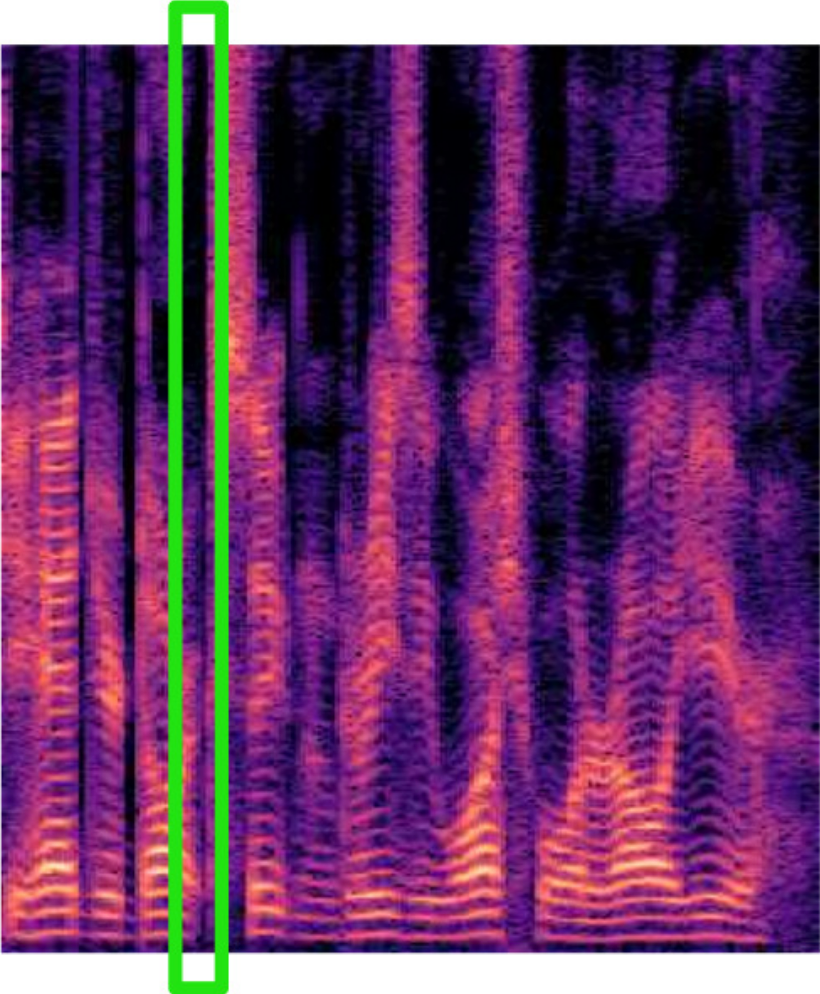
\includegraphics[width=.25\textwidth]{tikz/spectrogram}};
%   \node[inner sep=0pt,left of=encoder-1-1,xshift=-0.5cm,yshift=-2.4cm] (input2) {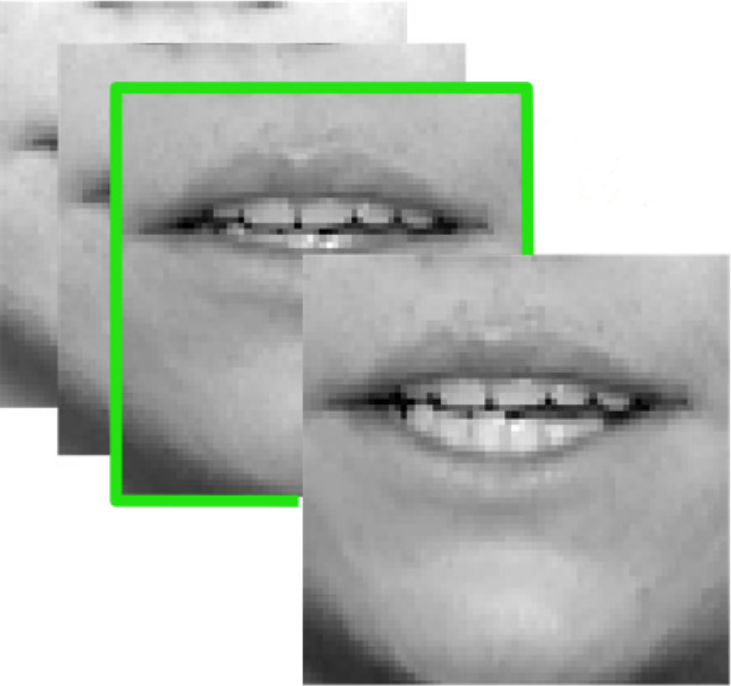
\includegraphics[width=.25\textwidth]{tikz/lips}};
  
  % mu, sigma, sample nodes, conditioning
  \foreach \idx in {1,...,3} {
%       \coordinate[neuron, right=2 of encoder-2-2, xshift=-1.4cm, yshift=0.5*\idx cm-0.15cm, fill=red, fill opacity=0.2] (mu-\idx);
%       \coordinate[neuron, right=2 of encoder-2-2, xshift=-1.4cm, yshift=-0.5*\idx cm+0.15cm, fill=red, fill opacity=0.2] (sigma-\idx);
      \coordinate[neuron, left=of decoder-a-1-\idx, xshift=6mm, fill=red, fill opacity=0.2] (sample-a-\idx);
      \coordinate[neuron, left=of decoder-av-1-1, xshift=6mm, yshift=0.5*\idx cm-0.4cm, fill=red, fill opacity=0.2] (sample-av-\idx);
      \coordinate[neuron, left=of decoder-av-1-1, xshift=6mm,yshift=0.5*\idx cm-2.3cm, fill=green, fill opacity=0.2] (cond-av-\idx);
    }
    
  \node[left=of sample-a-1,xshift=6mm,yshift=-2mm] (post-a) {\textcolor{blue}{Audio-only VAE}};
  \node[below=of post-a,yshift=1cm] {$q^a_{\bs{\phi}}(\bs{\mylz}_n|\bs{\myos}_n,\bs{\myov}_n)$};
  
  \node[left=of sample-av-3,xshift=6mm,yshift=-2mm] (post-av) {\textcolor{magenta}{Audio-Visual VAE}};
  \node[below=of post-av,yshift=1cm] {$q^{av}_{\bs{\phi}}(\bs{\mylz}_n|\bs{\myos}_n,\bs{\myov}_n)$};  
    
  \node[inner sep=0pt,left of=cond-av-1,xshift=-.5cm,yshift=5mm] (cond) {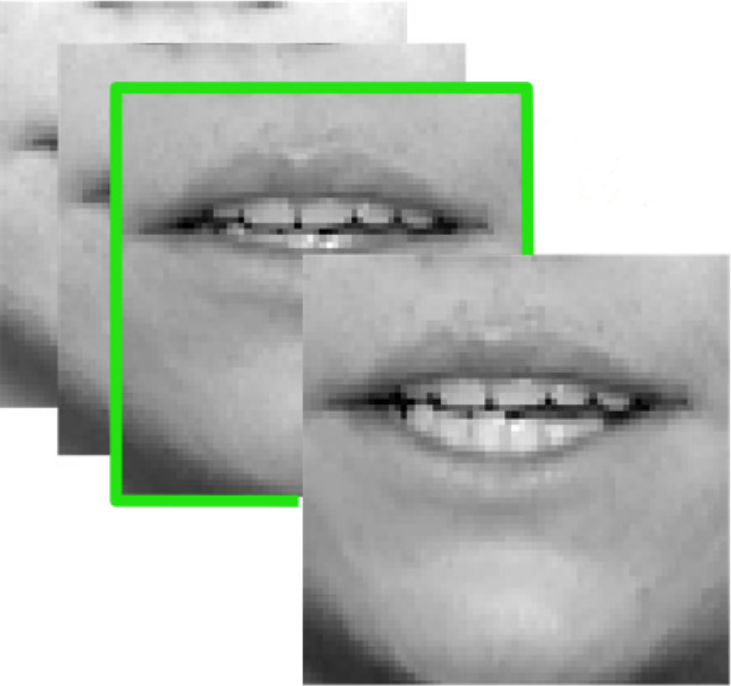
\includegraphics[width=.15\textwidth]{tikz/lips}};

  % mu, sigma, sample boxes
%   \node [label={above:$\bs{\mu}^{av}_{\bs{\mylz}}(\bs{\myos}_n,\bs{\myov}_n)$}, fit=(mu-1) (mu-3), draw] (mu) {};
%   \node [label={below:$\bs{\sigma}^{av}_{\bs{\mylz}}(\bs{\myos}_n,\bs{\myov}_n)$}, fit=(sigma-1) (sigma-3), draw] (sigma) {};
%   \node [fit=(sample-av-1) (sample-av-3), draw] (sample-av) {};
%   \node [fit=(sample-a-1) (sample-a-3), draw] (sample-a) {};

  \node [fit=(decoder-a-2-1) (decoder-a-2-4), draw] (decoder-a-2) {};
  \node [fit=(decoder-av-2-1) (decoder-av-2-4), draw] (decoder-av-2) {};
  \node [fit=(post-av) (sample-av-3) (cond-av-1) (decoder-av-2), draw=magenta, very thick] (vae-av) {};
  \node [fit=(post-a) (decoder-a-2), draw=blue, very thick] (vae-a) {};
  
  \node[circle,draw,below right=of decoder-a-2,yshift=9mm] (alpha) {$\bs{\alpha}_n$};
  \draw[->,blue] (vae-a.east) -- node[above,xshift=8mm] {$p_{\bs{\theta}}(\bs{\myos}_n|\bs{\mylz}^{a}_n)$} ++ (alpha);
  \draw[->,magenta] (vae-av.east) -- node[below,xshift=10mm] {$p_{\bs{\theta}}(\bs{\myos}_n|\bs{\mylz}^{av}_n,\bs{\myov}_n)$} ++ (alpha);
  % mu, sigma, sample connections
%   \draw[dashed] (mu.east) edge (sample.west) (sigma.east) -- (sample.west);
  \foreach \a in {1,2,3}
  \foreach \b in {1,2,3} {
%       \draw[-] (encoder-2-\a) -- (mu-\b);
      \draw[-] (sample-a-\a) -- (decoder-a-1-\b);
      \draw[-] (sample-av-\a) -- (decoder-av-1-\b);
      \draw[-] (cond-av-\a) -- (decoder-av-1-\b);
    }

    \node[inner sep=0pt,right of=alpha,xshift=1.5cm] (output) {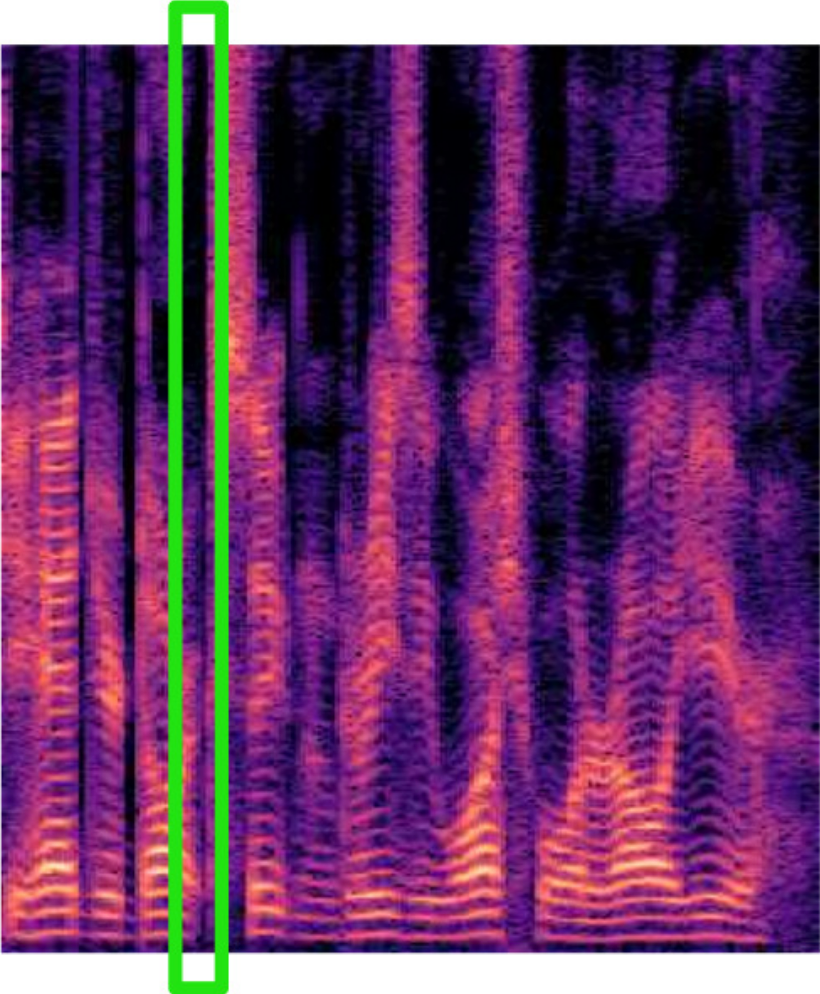
\includegraphics[width=.25\textwidth]{tikz/spectrogram}};
    \draw[->] (alpha) -- (output);
    
  % input + output labels
%   \foreach \idx in {1,...,4} {
%       \node[left=0 of encoder-1-\idx] {$x_\idx$};
%       \node[right=0 of decoder-2-\idx] {$\hat x_\idx$};
%     }
%   \node[above=0.1 of encoder-1-1] {$\bs{\myos}_n$};
%   \node[below=0.1 of encoder-1-6] {$\bs{\myov}_n$};
%   \node[above=0.1 of decoder-a-2-1] {$\hat{\bs{\myos}}_n$};
%   \node[below=0.1 of decoder-av-2-4] {$\hat{\bs{\myos}}_n$};

\end{tikzpicture}
}
  \end{column}
  \begin{column}{0.4\textwidth}
    $\bs{\alpha}_n$ is the ``mixing'' latent variable.\vspace{-2mm}
    \[\begin{cases}
       \bs{\alpha}_n=1 \leftrightarrow \text{\color{blue}Audio-only}\\
       \bs{\alpha}_n=0 \leftrightarrow \text{\color{magenta}Audio-Visual}
      \end{cases}\vspace{-2mm}
    \]
    Prior: $p(\alpha_n) = \textcolor{blue}{\pi}^{\alpha_n} (\textcolor{magenta}{1-\pi})^{1-\alpha_n}.$\vspace{8mm}\\
    The \textcolor{blue}{Audio-only} and the \textcolor{magenta}{Audio-Visual} VAE are \textbf{\alert{mixed without supervision}}.
  \end{column}
 \end{columns}
\end{frame}

%%%%%%%%%%%%%%%%%%%%%%%%%%%%%%%%%%%%%%%%%%%%%%%%%%%%%%%%%%%%%%%%%%%%%%%%%%%%
\begin{frame}{Train, adaptation \& speech enhancement}
\begin{columns}
\begin{column}{0.35\textwidth}
\begin{center}
\begin{tikzpicture}
% Audio-only (blue)
\node[det,draw=blue] (theta-a) {${\color{blue}\bs{\theta}^{a}}$};
\node[latent,below right=of theta-a,xshift=-1.5mm,yshift=5mm,draw=blue] (z-a) {$\bs{\mylz}^{\color{blue}a}$};
\node[latent,right=of theta-a,draw=blue,xshift=3mm] (s-a) {$\bs{\only<1>{\myos}\only<2->{\myls}}^{\color{blue}a}$};
\node[fit=(theta-a) (s-a) (z-a),draw=blue] (a-vae) {};
\edge[draw=blue]{theta-a} {s-a};
\edge[draw=blue] {theta-a} {z-a}; \edge[draw=blue]{z-a} {s-a};
% Audio-visual (magenta)
\node[det,below=of theta-a,draw=magenta,yshift=-1mm] (theta-av) {${\color{magenta}\bs{\theta}^{av}},\bs{\myov}$};
\node[latent,below right=of theta-av,xshift=-3mm,yshift=5mm,draw=magenta] (z-av) {$\bs{\mylz}^{\color{magenta}av}$};
\node[latent,right=of theta-av,draw=magenta] (s-av) {$\bs{\only<1>{\myos}\only<2->{\myls}}^{\color{magenta}av}$};
\node[fit=(theta-av) (s-av) (z-av),draw=magenta] (av-vae) {};
\edge[draw=magenta]{theta-av} {s-av};
\edge[draw=magenta] {theta-av} {z-av}; \edge[draw=magenta]{z-av} {s-av};
% Mixing variable
\only<2->{\node[latent,below right=of s-a,yshift=2mm] (s) {$\myls$};
\node[latent,above=of s,yshift=2mm] (alpha) {$\bs{\color{red}\alpha}$};
\edge[->]{s-a,s-av,alpha} {s};}
% Noise
\only<3->{\node[det,below=of theta-av] (eta) {$\alert{\bs{\psi}}$};
\node[latent,right=of eta,xshift=3mm] (b) {$\color{gray}\mathbf{b}$};
\node[fit=(eta) (b),draw] (a-vae) {};
\edge{eta} {b};}
% Combining
\only<4->{\node[latent,below=of s] (plus) {\Large$+$};
\node[obs,below=of plus] (x) {$\color{green}\mathbf{x}$};
\edge{s,b} {plus};
\edge{plus} {x};}

\end{tikzpicture}
\end{center}
\end{column}%
\begin{column}{0.7\textwidth}
 \begin{itemize}
  \item Train \textcolor{blue}{A-VAE} (with $\bs{\myos}$) and \textcolor{magenta}{AV-VAE} (with $(\bs{\myos},\bs{\myov})$).
  \item<2-> The clean speeh is now \textcolor{red}{latent} ($\bs{\myls}^{\color{blue}a}, \bs{\myls}^{\color{magenta}av}$), add the\\ \textcolor{red}{mixing latent} variable ($\bs{\color{red}\alpha}$).
  \item<3-> We also consider the noise variable and params.
  \item<4-> Learn $\alert{\bs{\psi}}^\ast$ and estimate the clean speech. \only<4->{By defining\\
  {\small$\bs{\gamma}_{n}(\bs{\mylz}_n,\bs{\myov}_n) = \left( {\color{blue}\pi_n} ({\color{blue}\bs{\sigma}^a_{s}(\bs{\mylz}_n)})^{-1} + ({\color{magenta}1-\pi_n})({\color{magenta}\bs{\sigma}^{av}_{s}(\bs{\mylz}_n,\bs{\myov}_n)})^{-1}\right)^{-1}$}}\only<5->{:
  \begin{align*}
\label{source_estimate}
\hat{\bs{s}}_{n}
&= \frac{1}{R}\sum_{r=1}^R  \frac{ \bs{\gamma}_{n}(\bs{\mylz}_n^{(r)},\bs{\myov}_n)}{
	\bs{\gamma}_{n}(\bs{\mylz}_n^{(r)},\bs{\myov}_n) + \bs{\alert{\psi}}^\ast_n}\,\bs{\myox}_{n}
\end{align*}}
 \end{itemize}
\end{column}
\end{columns}
\end{frame}

\begin{frame}{Learning the noise parameters with VAE-MM}
 \textbf{Ideally}:
\[Q(\bs{\psi},\bs{\psi}^0) = \sum_{n=1}^N\E_{\alert{p(\bs{s}_n, \bs{z}_n, \alpha_n|\mathbf{x}_n,\bs{v}_n;\bs{\psi}^0)}} [\log p(\mathbf{x}_n,\bs{s}_n, \bs{z}_n, \alpha_n|\bs{v}_n;\bs{\psi})]\]
We need to approximate this posterior:
\[p(\bs{s}_n, \bs{z}_n, \alpha_n|\mathbf{x}_n,\bs{v}_n;\bs{\psi}^0) \approx q(\bs{s}_n, \bs{z}_n, \alpha_n) = q_{\bs{s}}(\bs{s}_n)\; q_{\bs{z}}(\bs{z}_n)\; q_{\alpha}(\alpha_n).\]
Of course we will need to sample from $q_{\bs{z}}$, but in that case:
\begin{enumerate}
 \item $q_{\alpha}$ is a Bernoulli distribution.
 \item $q_{\bs{s}}$ is a complex Gaussian distribution.
\end{enumerate}

\end{frame}


%%%%%%%%%%%%%%%%%%%%%%%%%%%%%%%%%%%%%%%%%%%%%%%%%%%%%%%%%%%%%%%%%%%%%%%%%%%%
\begin{frame}{ML with latent variables: EM vs VAE?}
ML with latent variable ($\bs{z}$) leads to EM\footnote{Dempster, A.P., \textit{et. al.}, (1977), Journal of the Royal Statistical Society.} and VI\footnote{Jordan, M. I., \textit{et. al.}, (1999),. Machine Learning.} build from {\footnotesize($\color{blue}q(\bs{z})$ is an arbitrary distribution)}:
\begin{align*}
\log p(\bs{x}) &= \underbrace{\mathbb{E}_{\color{blue}q(\bs{z})}\Big[\log \frac{p(\bs{x})p(\bs{z}|\bs{x})}{\color{blue}q(\bs{z})}\Big]}_{\text{M-step or VLB}} +  \underbrace{D_{\text{KL}}\Big({\color{blue}q(\bs{z})}\Big\lVert p(\bs{z}|\bs{x})\Big)}_{\text{E-step}}
\end{align*}
\begin{columns}
 \begin{column}{0.31\textwidth}
  \centering
  \underline{Exact EM}\\
  Simple $p(\bs{z}|\bs{x})$ \\
  ${\color{blue}q(\bs{z})}=p(\bs{z}|\bs{x})$\\
  Closed-form!\\
  $D_{\text{KL}} = 0$
 \end{column}\visible<2>{%
 \begin{column}{0.31\textwidth}
 \centering
  \underline{Variational EM}\\
  $p(\bs{z}|\bs{x})$ comp. complex\\
  ${q([\bs{z}_1,\bs{z}_2]) = q_1(\bs{z}_1)q_2(\bs{z}_2)}$\\
  $q_1,q_2=\argmin D_{\text{KL}}$\\
  $D_{\text{KL}}>0$ but closed form!
 \end{column}}%
  \begin{column}{0.31\textwidth}
 \centering
  \underline{Variational AutoEncoder}\\
  $p(\bs{z}|\bs{x})$ ???\\
  ${\color{blue}q(\bs{z})} = q_{\bs{\phi}}(\bs{z})$\\
  $q_{\bs{\phi}}$ optimises ELBO/VLB\\
  $D_{\text{KL}}>0$ no closed form!
 \end{column}
\end{columns}
\end{frame}


\begin{frame}{Conclusions}
 \begin{itemize}
  \item Auditory and visual data have very different properties.
  \item It is important (in general) to understand if the network/method is provided with the right data and loss functions.
  \item Unsupervised probabilistic learning provides a nice generic framework, that declines in several types of models.
  \item Complex probabilistic models require approximations, and there are many possibilities to be explored.
 \end{itemize}
 %\vspace{1cm}
 
%  \alert{The mid-term exam will soon be availabe at \url{https://xavirema.eu/AMLSlides}.\\
%  Due on Jan 19th at noon! (Instructions provided in the PDF).}
\end{frame}


\end{document}

